\PassOptionsToPackage{expansion=false}{microtype}
\documentclass[sigconf]{acmart}
\usepackage{enumitem}
\usepackage{xspace}
\usepackage{tikz}
\usetikzlibrary{arrows.meta, calc, positioning, shapes.geometric, backgrounds, decorations.markings, fit}
\usepackage{pgfplots}
\pgfplotsset{compat=1.18}
\usepackage[table]{xcolor}
\usepackage{mdframed}

\newcommand{\stix}{STIX\xspace}
\newcommand{\mitre}{MITRE\xspace}
\newcommand{\attack}{ATT\&CK\xspace}
\newcommand{\caldera}{Caldera\xspace}
\newcommand{\myparagraph}[1]{\textbf{#1.}\hspace{0.5em}}

\newcommand{\stepone}{\textcircled{\scriptsize 1}}
\newcommand{\steptwo}{\textcircled{\scriptsize 2}}
\newcommand{\stepthree}{\textcircled{\scriptsize 3}}
\newcommand{\stepfour}{\textcircled{\scriptsize 4}}
\newcommand{\stepfive}{\textcircled{\scriptsize 5}}

% Measurement values for Paper 1 (STICKS Docker boundary)
% Bundle: sticks/data/stix/enterprise-attack.json
% Computed by: python3 sticks-docker/measurement/scripts/analyze_campaigns.py --bundle sticks/data/stix/enterprise-attack.json --output-latex
%
% Platform-agnostic techniques are active top-level ATT&CK techniques without
% a concrete host platform among Windows, Linux, macOS, Containers, ESXi,
% or Network Devices.

% --- Dataset counts ---
\newcommand{\nCampaignsTotal}{52}
\newcommand{\nCampaigns}{51}
\newcommand{\nIntrusionSets}{172}
\newcommand{\nRelationships}{17270}
\newcommand{\nAttackPatternObjects}{691}
\newcommand{\nTechniquesAnalysis}{691}
\newcommand{\nComposedObjects}{24772}

% --- Campaign technique coverage ---
\newcommand{\campaignCoveragePct}{43.0}
\newcommand{\campaignCoverageUnusedPct}{57.0}
\newcommand{\campaignTechniqueCount}{297}
\newcommand{\intrusionSetCoveragePct}{70.6}
\newcommand{\intrusionSetTechniqueCount}{488}
\newcommand{\sharedTechniqueCount}{268}
\newcommand{\campaignOnlyCount}{29}
\newcommand{\intrusionSetOnlyCount}{220}
\newcommand{\unusedTechniqueCount}{174}

% --- Venn diagram percentages ---
\newcommand{\campaignOnlyPct}{4.2}
\newcommand{\sharedPct}{38.8}
\newcommand{\intrusionSetOnlyPct}{31.8}
\newcommand{\unusedPct}{25.2}

% --- Technique frequency ---
\newcommand{\topTechniqueId}{T1105}
\newcommand{\topTechniqueLabel}{Ingress Tool Transfer}
\newcommand{\topTechniqueInCampaigns}{28}
\newcommand{\topTechniquePct}{55}

% --- Intrusion sets ---
\newcommand{\nIntrusionSetsWithTechniques}{168}
\newcommand{\intrusionSetWithTechniquesPct}{97.7}
\newcommand{\nIntrusionSetsEmpty}{4}
\newcommand{\intrusionSetEmptyPct}{2.3}
\newcommand{\intrusionSetTechRefs}{4362}
\newcommand{\intrusionSetTechAvg}{26.0}

% --- Emulation ---
\newcommand{\nPlatformAgnosticTechniques}{32}
\newcommand{\nTranslatableTechniques}{659}
\newcommand{\nCaseStudyCampaigns}{2}
\newcommand{\caseStudyRunsEach}{10}

% --- Clustering and LCS ---
\newcommand{\silhouetteScore}{0.05}
\newcommand{\silhouetteBaselineMean}{-0.01}
\newcommand{\silhouetteBaselineStd}{0.01}
\newcommand{\lcsLengthMean}{2.8}
\newcommand{\lcsLengthMedian}{2.0}
\newcommand{\lcsLengthMax}{29}

\newcommand{\nAppendixAttackPatterns}{691}
\newcommand{\AppendixFieldPopulationRows}{%
\texttt{kill\_chain\_phases} & 691 & 691 \\
\texttt{x\_mitre\_platforms} & 691 & 691 \\
\texttt{x\_mitre\_system\_requirements} & 0 & 0 \\
\texttt{x\_mitre\_detection} & 691 & 0 \\
\texttt{x\_mitre\_data\_sources} & 0 & 0 \\
\texttt{x\_mitre\_permissions\_required} & 0 & 0 \\
}
\newcommand{\AppendixItemsetRows}{%
1 & 28 & 54.9\% \\
2 & 17 & 33.3\% \\
3 & 10 & 19.6\% \\
4 & 7 & 13.7\% \\
5 & 6 & 11.8\% \\
}
\newcommand{\AppendixDockerRows}{%
APT41 DUST & 24 & Yes & 0 \\
C0010 & 10 & Yes & 0 \\
C0026 & 7 & Yes & 0 \\
CostaRicto & 11 & Yes & 0 \\
Operation MidnightEclipse & 18 & Yes & 0 \\
Outer Space & 9 & Yes & 0 \\
Salesforce Data Exfiltration & 19 & Yes & 0 \\
ShadowRay & 11 & Yes & 0 \\
}


% --- Okabe-Ito palette (colorblind-safe, ISO-recommended) -----------------
% Reference: Okabe & Ito 2008; recommended by Nature, Science, Cell.
% Unified across Paper 1 and Paper 2 for visual consistency.
\definecolor{execblue}{HTML}{1F77B4}   % primary data / structural elements
\definecolor{ctired}{HTML}{D55E00}     % alert / gap emphasis (vermillion)
\definecolor{loopgreen}{HTML}{009E73}  % automation / positive signal (bluish green)
\definecolor{tolyellow}{HTML}{E69F00}  % caution (spare — amber)
\definecolor{tolcyan}{HTML}{56B4E9}    % secondary accent (spare — sky blue)
\definecolor{tolpurple}{HTML}{CC79A7}  % tertiary accent (spare — reddish purple)
% --- Neutral grays (luminance-calibrated for hierarchy) ---
\definecolor{edgegray}{HTML}{333333}   % axes, borders, primary text in figs
\definecolor{midgray}{HTML}{666666}    % secondary text, annotations
\definecolor{dashgray}{HTML}{D9DDE2}   % grid lines, subtle dividers (cool-toned)
\definecolor{stagefill}{HTML}{F5F5F5}  % grouping backgrounds (minimal)
\definecolor{facegray}{HTML}{FFFFFF}   % plot backgrounds: always white
% --- Finding-box palette (consistent with figure palette) ---
\definecolor{findBlue}{HTML}{1F77B4}
\definecolor{findBg}{HTML}{E8F0F8}

\tikzset{
  computer/.pic={
    \draw[fill=dashgray!20, draw=edgegray!60, rounded corners=1.5pt,
          line width=0.5pt]
      (-0.55,-0.45) rectangle (0.55,0.45);
    \fill[dashgray!30] (-0.46,-0.36) rectangle (0.46,0.36);
    \draw[fill=edgegray!25, draw=edgegray!60, line width=0.5pt]
      (-0.12,-0.63) rectangle (0.12,-0.45);
    \draw[fill=edgegray!20, draw=edgegray!60, line width=0.5pt]
      (-0.33,-0.70) rectangle (0.33,-0.63);
  }
}

\newmdenv[
  topline=false, bottomline=false, rightline=false,
  linewidth=2.5pt, linecolor=findBlue,
  backgroundcolor=findBg,
  innerleftmargin=7pt, innerrightmargin=5pt,
  innertopmargin=4pt, innerbottommargin=4pt,
  skipabove=5pt, skipbelow=3pt
]{findingenv}
\newcommand{\finding}[2]{%
  \begin{findingenv}%
    \textsc{\textbf{Finding~#1.}}\enspace #2%
  \end{findingenv}%
}

\newmdenv[
  topline=true, bottomline=true, leftline=false, rightline=false,
  linewidth=0.6pt, linecolor=black!30,
  backgroundcolor=gray!5,
  innerleftmargin=6pt, innerrightmargin=6pt,
  innertopmargin=5pt, innerbottommargin=5pt,
  skipabove=6pt, skipbelow=4pt
]{textbox}

\setlength{\emergencystretch}{1.2em}

\AtBeginDocument{%
  \providecommand\BibTeX{{%
    Bib\TeX}}}

\setcopyright{none}
\copyrightyear{2026}
\acmYear{2026}
\acmDOI{}
\acmConference[ACM CCS '26]{2026 ACM SIGSAC Conference on Computer and Communications Security}{November 15--19, 2026}{The Hague, The Netherlands}
\acmISBN{}
\begin{document}
\title{The Procedural Semantics Gap in ATT\&CK-in-STIX: A Measurement-Driven Analysis for APT Emulation}
\author{Ágney Lopes Roth Ferraz}
\authornote{These authors contributed equally to this work.}
\orcid{0009-0009-1202-6447}
\affiliation{%
  \institution{Aeronautics Institute of Technology}
  \city{São José dos Campos}
  \state{SP}
  \country{Brazil}
}
\email{roth@ita.br}

\author{Sidnei Barbieri}
\authornotemark[1]
\orcid{0000-0001-9090-9469}
\affiliation{%
  \institution{Carnegie Mellon University}
  \city{Pittsburgh}
  \state{PA}
  \country{USA}
}
\additionalaffiliation{%
  \institution{Aeronautics Institute of Technology}
  \city{São José dos Campos}
  \state{SP}
  \country{Brazil}
}
\email{sbarbier@andrew.cmu.edu}

\author{Lourenço Alves Pereira Júnior}
\orcid{0000-0002-9682-0075}
\affiliation{%
  \institution{Aeronautics Institute of Technology}
  \city{São José dos Campos}
  \state{SP}
  \country{Brazil}
}
\email{ljr@ita.br}

\renewcommand{\shortauthors}{Ferraz et al.}

\begin{abstract}

Public \attack{} content serialized in Structured Threat Information Expression (\stix{}) has become a global reference for describing adversary behavior. Yet \attack{} was designed as a descriptive knowledge base, not as a procedural model. We therefore ask whether \attack{}-in-\stix{} contains enough behavioral detail to support multi-stage adversary emulation. Measuring the \attack{} Enterprise bundle, we find that campaign objects encode fragmented behavioral slices: only \campaignCoveragePct\% of techniques appear in at least one campaign, and neither clustering nor Longest Common Subsequence (LCS)-based probes reveal reusable structure. Intrusion sets cover more of the technique space, but still omit ordering, preconditions, and environmental assumptions. Public CTI therefore describes \emph{what} adversaries do, but not enough of \emph{how} to execute those behaviors automatically.

To test how far explicit translation can bridge that gap, we define a three-stage methodology and instantiate it in the \mitre{} \caldera{} framework. Case studies of \emph{ShadowRay} and \emph{Soft Cell} show that structured CTI can support multi-step adversary enactment only after missing parameters and assumptions are supplied and validated. We also audit the eight curated adversaries packaged in the legacy Docker artifact and find that all eight workflows reach explicit end markers within the observed window and leave no residual non-zero links once execution settles. Together, these results mark a reproducible boundary between behavioral signal already encoded in public CTI and the procedure that still must be supplied explicitly before execution.
\end{abstract}

\begin{CCSXML}
<ccs2012>
   <concept>
       <concept_id>10002978.10002997</concept_id>
       <concept_desc>Security and privacy~Intrusion/anomaly detection and malware mitigation</concept_desc>
       <concept_significance>500</concept_significance>
       </concept>
   <concept>
       <concept_id>10002978.10003006</concept_id>
       <concept_desc>Security and privacy~Systems security</concept_desc>
       <concept_significance>300</concept_significance>
       </concept>
   <concept>
       <concept_id>10002978.10003014</concept_id>
       <concept_desc>Security and privacy~Network security</concept_desc>
       <concept_significance>100</concept_significance>
       </concept>
 </ccs2012>
\end{CCSXML}

\ccsdesc[500]{Security and privacy~Intrusion/anomaly detection and malware mitigation}
\ccsdesc[300]{Security and privacy~Systems security}
\ccsdesc[100]{Security and privacy~Network security}

\keywords{cyber threat intelligence, STIX, MITRE ATT\&CK, system under test, adversary emulation, structured CTI}
\maketitle
\section{Introduction}\label{sec:introduction}

Advanced Persistent Threats (APTs) unfold as multi-stage campaigns that may span multiple hosts, adapt to the target environment, and frequently rely on “living-off-the-land” techniques that blend with legitimate activity~\cite{barr-smith2021survivalism}. Their distributed low-signal activities~\cite{lourenco2024devil} and prolonged dwell times~\cite{milajerdi2019holmes} make end-to-end reconstruction complex in Security Operations Centers (SOCs)~\cite{clearSkyFoxKitten,fireeyeAPT41,mandiant2025mtrends}.

Provenance-based detection and learning-driven approaches show why. Reconstructing multi-step behaviors induces dependency explosion and produces large provenance graphs with multiple roots~\cite{hossain202comb,10646673,10646725,zian2024magic}. They also show that short or synthetic traces fail to represent characteristic APT dependencies~\cite{milajerdi2019holmes,han2020unicorn,lourenco2024devil}.

Cyber Threat Intelligence (CTI) provides structured accounts of adversary tactics and techniques. Public feeds exhibit heterogeneous formats, uneven granularity, and inconsistent field usage~\cite{jin2024sharing,10117505}. However, extracting actionable information from narrative reports requires substantial manual effort~\cite{savat2021extractor}, and most CTI sources lack the procedural context and environmental constraints necessary for reproducible multi-host emulation~\cite{10117505}. Analyses of intrusion-detection rules additionally show rapid turnover, skewed alert distributions, and weak links between rules, alerts, and incidents~\cite{vermeer2022evolution}. As a result, CTI is used for mapping and coverage but rarely as a direct source of executable adversary actions.

The \mitre{} \attack{} framework provides a widely adopted taxonomy of tactics and techniques, disseminated as \stix{} bundles consumed by defensive platforms~\cite{apurva2024mitre,strom2018mitre,stixspec}. These bundles combine campaigns, intrusion sets, malware, tools, and relationships, but campaign and intrusion-set entries rarely encode temporal or causal information. Execution order, prerequisites, and environmental assumptions typically appear only in free text~\cite{stixspec,10117505,savat2021extractor}. Prior work either extracts partial behaviors from textual intelligence without producing executable actions~\cite{savat2021extractor,xu2024intelex,cheng2025ctinexus} or reconstructs long-duration campaigns from telemetry~\cite{lourenco2024devil,10646725,10646673}. The question of how far \attack{}-in-\stix{} can support APT emulation therefore remains open.

We intentionally study the Enterprise bundle because, among the public \stix{} sources we parsed, it preserves the most campaign-level structure. In our corpus, it is the source that most consistently combines campaigns, intrusion sets, techniques, and relationships in one bundle. If reusable procedural structure is weak even there, it is unlikely to be stronger or more consistent in sparser heterogeneous feeds.

Frameworks such as \mitre{} \caldera{} provide an execution substrate for emulating adversary behavior, but they do not supply the missing procedure. Analysts still have to infer ordering, bind parameters to a declared \emph{System Under Test (SUT)}, and discover during execution which assumptions were wrong~\cite{singer2025incalmo}. We therefore target the analyst, emulation engineer, or artifact author who wants to turn public structured CTI plus a declared SUT into an executable workflow without overstating historical fidelity. We ask which parts of that workflow are already encoded in public structured CTI, which still must be supplied, and how to distinguish the two. This framing motivates the central questions guiding this study:

\noindent\hangindent=2.7em\hangafter=1
\textbf{RQ1:} How much adversarial behavior do current \attack{}-in-\stix{} artifacts capture for multi-step APT emulation?

\noindent\hangindent=2.7em\hangafter=1
\textbf{RQ2:} How can structured CTI be transformed into computable multi-stage behavioral plans for emulation?

\noindent\hangindent=2.7em\hangafter=1
\textbf{RQ3:} Which structural and semantic gaps in descriptive CTI prevent automation, and how can they be mitigated?

Our contributions are fourfold. \stepone\ We measure coverage, sparsity, overlap, and clustering in the \mitre{} \attack{} Enterprise bundle and show that campaign objects expose narrow, heterogeneous slices of behavior rather than reusable procedural backbones. \steptwo\ We show that campaign and intrusion-set associations do not supply the ordering, preconditions, or environment bindings needed for multi-stage execution. \stepthree\ We define a three-stage translation methodology that makes the automation boundary explicit: structural modeling is automated, technique translation is analyst-supervised, and execution is scripted once steps are fixed. \stepfour\ We corroborate that boundary with two focal case studies and an eight-adversary Docker audit, distinguishing reproducible execution progress from campaign-isolated replay. Together, these results show that public \attack{}-in-\stix{} contains enough behavioral signal to ground enactment, but too little procedure to execute on its own.

Operationally, the input to our process is public structured CTI plus a declared SUT, and the output is an executable workflow together with an explicit record of the parameters, bindings, and assumptions that CTI did not provide. Success is therefore not historical replay, but a reproducible separation between the behavioral structure already encoded in CTI and the procedure that still must be added before execution.

\section{Background}
\label{sec:background}

CTI refers to evidence-based knowledge about cyber threats, ranging from low-level artifacts (IoCs) to descriptions of tactics, techniques, and procedures (TTPs). In its unstructured form, CTI appears as narrative reports, blog posts, and vendor documents, which require manual normalization before they can be used systematically. \stix{} was introduced to reduce that heterogeneity by standardizing threat entities and relationships in a machine-readable format~\cite{stixspec}. For this study, the relevant object types are attack-pattern, campaign, intrusion-set, malware, tool, and relationship. They capture behavioral entities and associations, but not, on their own, a campaign procedure chain.

Other structured models such as MISP and CASE make different trade-offs between simplicity and expressivity. We focus on \attack{}-in-\stix{} because it remains the most widely adopted public representation of adversary behavior for cross-organizational CTI exchange and threat-informed defense~\cite{jin2024sharing,stixspec}.

\mitre{} maintains the \attack{} framework as a hierarchical knowledge base of TTPs observed in real campaigns, organized into matrices for different domains (Enterprise, Mobile, and ICS)~\cite{strom2018mitre}. In this taxonomy, \emph{tactics} capture objectives, while \emph{techniques} and \emph{sub-techniques} describe modes of operation. Beyond the matrix itself, \attack{} also indexes threat groups, campaigns, malware, tools, telemetry sources, and mitigations~\cite{strom2018mitre}. \mitre{} publishes this content as \stix{} bundles built from object types such as attack-pattern, intrusion-set, campaign, malware, tool, and relationship.

The conceptual layers are different. \attack{} is the ontology of adversary behavior, \stix{} is the serialization language used to publish it, and the Enterprise bundle is one concrete \stix{} export in the broader CTI ecosystem. In \attack{}, each technique or sub-technique is represented by an attack-pattern object with fields such as description, kill-chain phases, external references, and tactic mappings. These objects are the main building blocks used by extraction pipelines to align narrative reports with standardized technique identifiers~\cite{10117505,savat2021extractor,marvin2025sokttp}.

Objects of type \texttt{campaign} represent specific operations attributed to a threat actor. They typically encode time windows, objectives, targeted sectors, and a subset of associated techniques, malware, or tools. In practice, however, CTI feeds rarely enumerate all steps, prerequisites, or action sequences. Threat reports often omit steps, merge phases, or present only fragments of the intrusion~\cite{savat2021extractor}, and large-scale measurements report inconsistent field usage and heterogeneous reporting practices across providers~\cite{jin2024sharing}. As a result, campaigns encoded in \stix{} tend to lack the procedural specificity required for direct replay.

Objects of type \texttt{intrusion-set} aggregate the long-term behavior of a threat group across multiple campaigns, including commonly used malware, techniques, infrastructure, and motivations~\cite{abdulellah2021atlas}. In open \stix{} collections, campaigns are linked to intrusion sets via \texttt{relationship} objects that encode attribution, tool usage, or technique associations. This modeling reflects a common CTI distinction: \emph{intrusion sets} capture the persistent adversary profile, while \emph{campaigns} represent concrete operational instances. Even then, actor and technique labels remain inconsistent across vendors, which reduces interoperability~\cite{vermeer2022evolution}.

Despite its broad adoption, the \stix{} data model was designed to describe threat entities and relationships, not to reconstruct multi-host adversary behavior automatically~\cite{stixspec}. Although \attack{}-in-\stix{} provides structured identifiers for techniques, tactics, campaigns, and intrusion sets, it does not directly encode temporal order, explicit prerequisites, detailed environmental constraints, or branching logic. Relationship objects can state that an intrusion set ``uses'' a malware family or that a campaign is ``attributed to'' a group, but they do not specify how to chain those entities into an execution plan. Graphs built from these bundles therefore capture \emph{which} entities are linked, not \emph{how} to replay a campaign chain~\cite{strom2018mitre,10117505,savat2021extractor}.

Open CTI collections also exhibit low coverage, delayed sharing, uneven field usage, and inconsistent labels~\cite{jin2024sharing,vermeer2022evolution}. Extraction pipelines can recover partial behaviors from reports, but they still do not yield executable sequences with preconditions, parameters, control logic, and SUT bindings~\cite{savat2021extractor,10117505,marvin2025sokttp,xu2024intelex,cheng2025ctinexus,deng2024raconteur}. Even when emulation tools such as \caldera{} are used, CTI descriptions still have to be transformed into ordered, parameterized plans, and current artifacts provide no formal SUT abstraction tying techniques to the environments in which they are expected to execute~\cite{apurva2024mitre,10.1145/3634737.3645012,singer2025incalmo}.

\section{Related Work}
\label{sec:related}

Recent advances in structured threat intelligence, technique extraction, and adversary emulation have expanded the range of available methodologies. Prior work analyzes the structure and quality of CTI feeds published in \stix{}, including aspects such as heterogeneity, coverage, and field consistency, as well as their impact on commercial platforms and detection evaluations~\cite{stixspec,jin2024sharing,10117505,strom2018mitre,apurva2024mitre,10.1145/3634737.3645012,vermeer2022evolution}. These studies quantify inconsistencies in field usage, rule annotations, and sharing practices, and show that both \attack{}-annotated rules and other \stix{} sources suffer from uneven coverage and vendor-specific practices. However, they do not assess whether public bundles contain sufficient procedural information to support multi-host emulation without analyst reconstruction, nor do they systematically investigate sequencing, operational dependencies, or the environmental context required for direct execution. As a result, existing work falls short of directly converting descriptive CTI into executable multi-step representations, motivating the approach developed in this paper.

Solutions for deriving adversary behavior from unstructured text, such as Extractor~\cite{savat2021extractor}, CTI HAL~\cite{dellapenna2025ctihal}, and NLP-based extraction pipelines~\cite{gabrys2024nlp,marvin2025sokttp,xu2024intelex,cheng2025ctinexus}, as well as LLM-powered command and script reasoning~\cite{deng2024raconteur}, advance the identification and organization of techniques, entities, and relationships. These approaches include supervised and weakly supervised extraction, Systematization of Knowledge (SoK)-style evaluations of TTP extraction quality, and LLM-based knowledge graph construction from CTI. However, they do not directly produce executable sequences from the structure already present in CTI bundles. They evaluate extraction quality rather than the completeness and sufficiency of the procedural structure encoded in \stix{} itself. Temporal relationships and execution conditions are inferred from narrative descriptions rather than assessed against the actual encoding in \stix{} bundles.

Closer in spirit to our measurement framing, Saha et al.~\cite{saha2026kitten} study how distinctive public threat-group profiles are for attribution. They show that only a minority of \attack{} groups have group-specific techniques, and that software often provides stronger group-level signatures than techniques alone. Our setting is complementary rather than contradictory. We focus on campaign and intrusion-set profiles inside the Enterprise bundle and compute exact positive-evidence witnesses and subsumption cases in that corpus. We then ask a different systems question: even when a profile is distinctive enough to separate one campaign or group from another, does the underlying \stix{} representation contain the procedural semantics needed to execute it? Their work clarifies the limits of attribution specificity; ours clarifies the limits of procedural sufficiency for emulation.

In the field of detection and investigation, telemetry- and provenance-based systems use \attack{} as an annotation taxonomy but reconstruct attack structure from logs rather than from CTI. Provenance-based detectors such as HOLMES, UNICORN, and ATLAS~\cite{milajerdi2019holmes,han2020unicorn,abdulellah2021atlas}, followed by ALchemist and NODLINK~\cite{yu2021alchemist,li2024nodlink}, show that correlating whole-system audit data is effective for reconstructing APT campaigns. Later work on provenance graph learning and scalable detection, including Flash, Kairos, DistDet, PROGRAPHER, and ProvG-Searcher~\cite{10646725,10646673,feng2023distdet,fanyang2023prographer,altinisik2023provg}, improves efficiency and search over large graphs.

Other approaches focus on tactic and technique recognition or online segmentation, such as TREC, TAPAS, SLOT, and OCR-APT~\cite{lv2024trec,zhang2025tapas,qiao2025slot,aly2025ocrapt}, or address lateral movement detection in temporal network graphs~\cite{king2023euler,khoury2024jbeil}. Complementary measurements highlight practical and industrial aspects of provenance-based EDR and auditing, including operating costs, triage effort, and logging limitations~\cite{dong2023arewe,jiang2023auditing}. Together, these works provide detailed visibility into campaign behavior and operational constraints, but they do not treat \stix{} as a primary procedural source for emulation: the attack chains are reconstructed from telemetry rather than derived from CTI object structures.

Adversary emulation frameworks such as Laccolith~\cite{orbinato2024laccolith}, PentestGPT~\cite{deng2024pentestgpt}, PentestAgent~\cite{shen2025pentestagent}, and language model-driven proposals for offensive planning and cyber deception~\cite{singer2025incalmo,singer2025perry} rely on curated procedures, environment models, and execution logic that specify ordering, preconditions, and cleanup. Their evaluations are conducted on fixed or parameterized SUTs, often using standardized lab topologies or web application environments as benchmarks. This shows that reproducibility depends on the description of attacker behavior and on explicit specification of the SUT. In particular, PentestGPT studies LLM-guided offensive interaction on benchmark targets, while InCALMO targets more autonomous multi-host operation through an explicit action layer.

Closely related standardization efforts already move in the same direction: OASIS CACAO playbooks~\cite{cacao2spec} provide a shareable format for security workflows, and MITRE CTID Attack Flow~\cite{attackflowctid} explicitly represents flows of \attack{} techniques. Our setting is narrower and more diagnostic: we ask what fraction of that procedural burden can be derived from \stix{} itself before any analyst- or model-assisted translation layer is applied. Structured CTI provides technique identifiers and high-level behavioral context but still requires an additional translation step before it can be executed as a multi-stage procedure. We therefore evaluate the extent to which current \stix{}-encoded \attack{} data contains, or lacks, the procedural semantics required for machine-actionable emulation.

Frameworks that operationalize adversary behavior help clarify what structured CTI does and does not provide. Planning-based systems such as AURORA~\cite{wang2024sands} model actions through explicit preconditions and effects; the Effects Language (EL) formalism~\cite{damodaran2025automated} demonstrates that executable coordination requires ordering and guarded effects; and knowledge graph approaches such as KNOWHOW~\cite{meng2025knowhow} and MultiKG~\cite{wang2024multikg} enrich CTI with structure derived from telemetry or cross-source aggregation. These systems rely on procedural elements (ordering, parameters, bindings, and environment assumptions) that are not encoded in the current \mitre{} \attack{} Enterprise bundle. Our methodology is therefore complementary: it identifies the procedural information missing from this bundle. It shows how descriptive CTI can be converted into representations suitable for multi-host emulation, while explicitly characterizing what current standards cannot automate. Additionally, to our knowledge, no prior work treats the \attack{} Enterprise bundle itself as the object of measurement to assess its suitability for machine-actionable multi-step emulation.

\section{Behavioral Metrics}
\label{sec:definitions}

\begin{table*}[!t]
  \caption{\stix{} sources in the consolidated dataset.}
  \label{tab:sources}
  \centering
  \small
  \begin{tabular}{@{}lccccl@{}}
    \toprule
    Source & Type & Objects & Unique & Duplicates & Description \\
    \midrule
    \mitre{} Enterprise dataset & Repository & 24,771 & 24,771 & 0.0\% & Broad collection including TTPs, adversaries, and campaigns. \\
    \mitre{} CAPEC & Repository & 2,666 & 2,666 & 0.0\% & Attack patterns. \\
    DigitalSide & Repository & 38,306 & 38,306 & 0.0\% & Indicators, techniques, relationships, and malware with IOC focus. \\
    AlienVault OTX & TAXII server & 17,303 & 17,303 & 0.0\% & Diverse objects including \texttt{attack-pattern} and \texttt{threat-actor}. \\
    EclecticIQ & TAXII server & 2,335 & 2,043 & 12.5\% & Threat actors, campaigns, and reports. \\
    \midrule
    \textbf{Total (deduplicated)} & & \textbf{85,381} & \textbf{85,089} & 0.0\% & Nearly duplicate-free consolidated dataset. \\
    \bottomrule
  \end{tabular}
\end{table*}

Our analysis is supported by two components: the structure of \stix{} objects representing intrusion sets, campaigns, and techniques, and a set of quantitative measures derived from binary representations of technique usage. In the \mitre{} \attack{} Enterprise, adversary behavior is expressed as a heterogeneous graph of typed objects. The main behavioral entities considered here are attack-pattern (techniques and sub-techniques), x-mitre-tactic (tactics), campaign, intrusion-set, malware, tool, course-of-action, and relationship. Auxiliary entities such as indicator, identity, report, note, and x-mitre-data-source provide contextual metadata but do not encode procedural behavior. Table~\ref{tab:sources} lists the freely available \stix{} sources included in the consolidated dataset.

Before our qualitative evaluation, we first quantitatively characterize these entities. Attack-pattern objects represent techniques and sub-techniques, and the subtechnique-of relationship encodes their hierarchy. Tactics are represented by x-mitre-tactic objects and are referenced by techniques through the kill\_chain\_phases field. The \stix{} schema does not include dedicated fields for procedural information; ordering, preconditions, environmental requirements, dependencies, and parameter flows remain in natural-language descriptions and are not machine-readable. For the quantitative analysis, each campaign is encoded as a binary vector that indicates the presence or absence of each \attack{} technique. We choose the four metrics below because they probe complementary properties of reusable structure: breadth of documented behavior, matrix sparsity, pairwise reuse, and cluster cohesion.

\begin{textbox}
\textbf{Behavioral Metrics.}
Coverage: fraction of techniques and sub-techniques observed at least once across campaigns;
Sparsity: proportion of zero entries in the campaign-technique matrix;
Overlap: similarity between campaigns computed from shared techniques;
Clustering: stability of structural patterns measured by the \emph{silhouette} coefficient.
\end{textbox}

\section{Data Sources}
\label{sec:dataset}

The selected dataset is the Enterprise bundle of \mitre{} \attack{} in \stix{} format. It serves as the primary source of structured CTI for this study because it is publicly available, widely used in practice, and free of usage restrictions. \mitre{} distributes \attack{} datasets for the Enterprise, Mobile, and ICS domains, all encoded in \stix{}, and the additional CTI collections examined here also follow the \stix{} object model. \attack{} is commonly used to structure CTI and is relied upon by platforms such as Microsoft Sentinel, Microsoft Defender\footnote{Available at: \url{https://learn.microsoft.com/en-us/azure/sentinel/mitre-coverage?tabs=defender-portal}}, Falcon\footnote{Available at: \url{https://www.crowdstrike.com/en-us/press-releases/crowdstrike-achieves-100-percent-mitre-engenuity-attack-enterprise-evaluation/}}, and government initiatives such as CISA\footnote{Available at: \url{https://www.cisa.gov/news-events/news/best-practices-mitre-attckr-mapping}}.

We use this bundle (v18.1) as the authoritative source for all quantitative analyses in this study~\cite{strom2018mitre}. Additional non-versioned CTI sources were retrieved on 28 November 2025. Table~\ref{tab:sources} lists the objects obtained from each provider. The dataset will be released publicly after the completion of the double-blind review process. Although several feeds describe themselves as TTP collections, \stix{} does not define a structured procedure object; procedural behavior must therefore be reconstructed from contextual relationships such as \textit{uses}, \textit{attributed-to}, \textit{targets}, \textit{delivers}, and \textit{executes}, or from narrative descriptions, particularly those found in campaign objects.

To ensure reproducibility, we specify the object counts used in our analysis. The Enterprise bundle contains 52 campaign SDOs, but one (C0033) lacks any \textit{uses} relationships and is excluded, leaving 51 campaigns. The bundle includes 20,048 relationship objects in total, of which \nRelationships{} are \textit{uses} relationships relevant to the behavioral links analyzed here. At the attack-pattern layer, the raw bundle exposes 835 \attack{} technique or sub-technique objects with \texttt{T...} identifiers; 144 are revoked or deprecated, leaving the \nAttackPatternObjects{} active attack-pattern objects with behavioral content used in our quantitative metrics. All quantitative analyses presented in this paper (coverage, sparsity, overlap, clustering, campaign-group alignment) are computed exclusively on the Enterprise bundle.

We process \stix{} 2.x objects representing APT groups, their campaigns, observed behaviors, infrastructure, and kill-chain elements. This dataset catalogs indicators, tools, techniques, and sub-techniques, along with their associations with campaigns and intrusion sets. These objects provide structured entities and links, but not execution logic, ordering, or temporal constraints. We also performed a deduplication analysis using multiple comparison criteria across \stix{} objects. Apart from expected duplication in the EclecticIQ source, no redundant entries were found. The consolidated dataset contains 85,089 distinct objects.

\begin{figure*}[!t]
  \centering
  \resizebox{\textwidth}{!}{% methodology.tex — Three-stage methodology pipeline
% Design goal: austere, full-width conceptual pipeline with explicit geometry.
% Host requirement: the parent document must load TikZ.
\usetikzlibrary{arrows.meta,calc,shapes.geometric}%
\providecolor{execblue}{HTML}{1F77B4}%
\providecolor{ctired}{HTML}{D55E00}%
\providecolor{loopgreen}{HTML}{009E73}%
\providecolor{midgray}{HTML}{666666}%
\providecolor{dashgray}{HTML}{D9DDE2}%
\providecolor{edgegray}{HTML}{333333}%
\providecolor{facegray}{HTML}{FFFFFF}%
\providecolor{stagefill}{HTML}{F5F5F5}%
\providecommand{\stix}{STIX}%
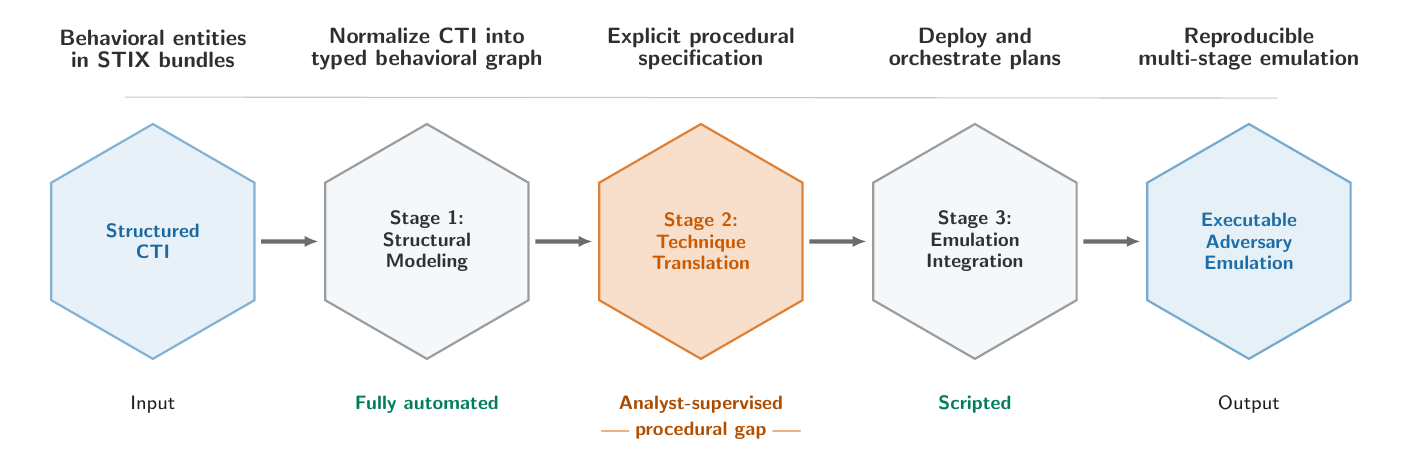
\begin{tikzpicture}[
  x=1cm,y=1cm,
  font=\sffamily\footnotesize,
  hex/.style={
    shape=regular polygon,
    regular polygon sides=6,
    shape border rotate=30,
    minimum size=2.16cm,
    text width=1.70cm,
    inner sep=1.8pt,
    align=center,
    line width=0.80pt,
    fill=execblue!5,
    draw=edgegray!48,
    text=edgegray!96!black,
    font=\sffamily\bfseries\fontsize{7.40}{7.80}\selectfont
  },
  hexfirst/.style={hex, fill=execblue!10, draw=execblue!56, text=execblue!88!black},
  hexexec/.style={hex, fill=execblue!11, draw=execblue!62, text=execblue!92!black},
  hexgap/.style={hex, fill=ctired!20, draw=ctired!78, text=ctired!95!black},
  arrow/.style={
    -{Latex[length=5.0pt,width=4.1pt]},
    line width=1.52pt,
    draw=edgegray!72
  },
  toplabel/.style={
    font=\sffamily\bfseries\fontsize{7.60}{8.10}\selectfont,
    text=edgegray!92!black,
    align=center,
    text width=3.18cm,
    inner sep=0pt
  },
  statelab/.style={
    font=\sffamily\bfseries\fontsize{7.40}{7.90}\selectfont,
    align=center,
    inner sep=0pt,
    text=loopgreen!80!black
  },
  analystlab/.style={
    font=\sffamily\bfseries\fontsize{7.40}{7.90}\selectfont,
    align=center,
    inner sep=0pt,
    text=ctired!80!black
  },
  rolelab/.style={
    font=\sffamily\fontsize{6.90}{7.30}\selectfont,
    align=center,
    inner sep=0pt,
    text=edgegray!58!black
  }
]

\def\yHex{0}
\def\xFirst{1.08}
\def\xStep{3.48}

% --- Stage centers --------------------------------------------------------
\coordinate (c1) at (\xFirst,\yHex);
\coordinate (c2) at ({\xFirst+\xStep},\yHex);
\coordinate (c3) at ({\xFirst+2*\xStep},\yHex);
\coordinate (c4) at ({\xFirst+3*\xStep},\yHex);
\coordinate (c5) at ({\xFirst+4*\xStep},\yHex);

% --- Hexagons -------------------------------------------------------------
\node[hexfirst] (cti)  at (c1) {Structured\\CTI};
\node[hex] (s1) at (c2) {Stage 1:\\Structural\\Modeling};
\node[hexgap] (s2) at (c3) {Stage 2:\\Technique\\Translation};
\node[hex] (s3) at (c4) {Stage 3:\\Emulation\\Integration};
\node[hexexec] (exec) at (c5) {Executable\\Adversary\\Emulation};

% --- Arrows between stages ------------------------------------------------
\draw[arrow] ([xshift=2pt]cti.east) -- ([xshift=-2pt]s1.west);
\draw[arrow] ([xshift=2pt]s1.east)  -- ([xshift=-2pt]s2.west);
\draw[arrow] ([xshift=2pt]s2.east)  -- ([xshift=-2pt]s3.west);
\draw[arrow] ([xshift=2pt]s3.east)  -- ([xshift=-2pt]exec.west);

% --- Top annotations ------------------------------------------------------
\node[toplabel] (ann1) at ($(cti.north)+(0,0.94cm)$)  {Behavioral entities\\in \stix{} bundles};
\node[toplabel] (ann2) at ($(s1.north)+(0,0.94cm)$)   {Normalize CTI into\\typed behavioral graph};
\node[toplabel] (ann3) at ($(s2.north)+(0,0.94cm)$)   {Explicit procedural\\specification};
\node[toplabel] (ann4) at ($(s3.north)+(0,0.94cm)$)   {Deploy and\\orchestrate plans};
\node[toplabel] (ann5) at ($(exec.north)+(0,0.94cm)$) {Reproducible\\multi-stage emulation};

% Guide line between labels and hexagons
\draw[line width=0.40pt, draw=edgegray!28]
  ($(ann1.south)!0.53!(cti.north)+(-0.36cm,0)$) --
  ($(ann5.south)!0.53!(exec.north)+(0.36cm,0)$);

% --- Automation boundary labels --------------------------------------------
\node[statelab]   (auto1) at ($(s1.south)+(0,-0.56cm)$) {Fully automated};
\node[analystlab] (auto2) at ($(s2.south)+(0,-0.56cm)$) {Analyst-supervised};
\node[statelab]   (auto3) at ($(s3.south)+(0,-0.56cm)$) {Scripted};

% --- Role labels under input/output (subtle, for visual balance) -----------
\node[rolelab] at ($(cti.south)+(0,-0.56cm)$) {Input};
\node[rolelab] at ($(exec.south)+(0,-0.56cm)$) {Output};

% --- Procedural gap annotation (prominent — key contribution) --------------
\node[
  font=\sffamily\bfseries\itshape\fontsize{7.40}{7.80}\selectfont,
  text=ctired!84!black,
  inner sep=0pt,
  align=center
] (gaptext) at ($(auto2.south)+(0,-0.22cm)$) {procedural gap};

\draw[line width=0.80pt, draw=ctired!48, line cap=round]
  ($(gaptext.west)+(-0.42cm,0)$) -- ($(gaptext.west)+(-0.08cm,0)$);
\draw[line width=0.80pt, draw=ctired!48, line cap=round]
  ($(gaptext.east)+(0.08cm,0)$) -- ($(gaptext.east)+(0.42cm,0)$);

\end{tikzpicture}%
}
  \caption{High-level structure of the methodology to convert descriptive CTI into executable multi-stage adversary behavior.}
  \Description{High-level structure of the methodology to convert descriptive CTI into executable multi-stage adversary behavior.}
  \label{fig:methodology-overview}
\end{figure*}

For the specific goal of this work, systematic behavioral analysis and subsequent adversary emulation, we therefore restrict campaign-level quantitative analysis to the \attack{} Enterprise subset. The remaining \stix{} sources are used only to characterize ecosystem-level diversity and coverage. In our parsed public-source corpus, Enterprise preserved the richest campaign-level behavioral structure, making it the most informative public baseline for procedural-sufficiency measurement.


\section{Methodology}
\label{sec:methodology}

To evaluate whether structured threat intelligence can be transformed into machine-actionable representations for multi-stage adversary emulation, we propose a three-stage methodology defined at an abstract level. The approach is format- and platform-agnostic, requiring only structured behavioral entities and explicit relationships among them. In this work, we instantiate the methodology using \stix{}~2.1 objects and the \caldera{} framework to show how the three stages map onto a concrete toolchain.

Figure~\ref{fig:methodology-overview} presents the three conceptual stages of the methodology. Stage~1 performs automated structural modeling of CTI data. Stage~2 introduces an analyst-supervised translation from abstract behavioral descriptions to minimal executable steps. This translation can be assisted by public templates or language models, but it is always validated against the source CTI and the target environment. Stage~3 integrates these steps into an emulation environment. In the instantiation studied here, the automation boundary is explicit: Stage~1 is fully automated, Stage~2 is analyst-supervised, and Stage~3 is scripted once the translated steps are fixed. The figure is conceptual rather than an implementation diagram and does not assume any specific serialization.


\subsection{Stage~1: Automated Structural Modeling}
\label{sec:stage1}

Structured CTI is modeled as a typed behavioral graph, where nodes represent entities such as techniques, campaigns, intrusion sets, malware, and tools, and edges encode relations such as \texttt{uses}, \texttt{attributed-to}, and \texttt{subtechnique-of}. Any CTI representation that exposes typed objects and explicit relationship fields can be normalized into this form. Each behavioral entity is mapped into a uniform internal representation. Techniques or equivalent abstractions are encoded as elements of a fixed behavioral space. Campaigns or long-term threat operations are represented as binary or categorical vectors denoting the presence of relevant techniques. Relationships are translated into vector entries.

Because structured CTI generally lacks explicit temporal or causal ordering, we derive a conservative tactic-ordered list for each campaign or intrusion set by aligning each technique with its associated \attack{} tactic and placing it along the canonical progression from Reconnaissance to Impact. Since a technique may be related to multiple tactics via the \texttt{kill\_chain\_phases} field, we assign it to one tactic by selecting the earliest tactic in this canonical order, with remaining ties broken deterministically using the technique's external identifier. This ordering is used strictly as an organizational scaffold rather than as a temporal or causal sequence. The scaffold provides a stable organizational backbone without introducing procedural semantics absent from the original CTI.

Sequence-comparison analyses (e.g., LCS) over these lists later test whether campaigns exhibit stable, reusable chains of techniques. Stage~1 yields a normalized behavioral graph, matrices linking campaigns or threat groups to techniques, and tactic-ordered technique lists that serve as structural scaffolding for subsequent stages.

\subsection{Stage~2: Technique Translation Layer}
\label{sec:stage2}

Stage~2 bridges the gap between high-level behavioral descriptions and executable steps. Existing CTI typically states \emph{what} occurred, not \emph{how}, and therefore lacks the procedural semantics needed for automation. Some interpretation is required to fill this gap.

Stage~2 operates on a campaign's tactic-ordered technique list rather than on the raw order of bundle objects. For orientation, Figure~\ref{fig:full_chart} summarizes attack-pattern counts in the composed corpus after assigning each object to one tactic bin for visualization and placing the bins in the canonical \attack{} Enterprise tactic order; the translation itself uses only the \nAttackPatternObjects{} Enterprise attack-patterns with behavioral content. For each technique in the tactic-ordered list, we extract the behavior implied by the structured representation and check whether prior examples or public repositories (e.g., Atomic Red Team - ART) offer templates. We optionally use language-model assistance to draft candidate commands and then refine the action against platform constraints, privilege requirements, and environmental assumptions.

The result is an executable step that captures the intended behavior without contradicting the available intelligence. When parameters, preconditions, or environmental bindings are absent from the structured input, we document them explicitly. We also record lightweight provenance to preserve traceability between CTI entities and the resulting steps. Stage~2 therefore produces context-aware executable steps together with explicit documentation of assumptions and provenance.

A concrete example illustrates the role of Stage~2. In ShadowRay, structured CTI and \attack{} identify \texttt{T1190} (Exploit Public-Facing Application) and describe abuse of exposed Ray services, but they do not specify the exact endpoint, parameters, or success check needed in the laboratory SUT. A Stage~2 seed can therefore start from a generic template or placeholder command and then be bound to the environment by the analyst. In our Docker-backed instantiation, this binding yielded the concrete command \texttt{curl -X POST -F 'cmd=whoami' http://172.21.0.20:5055/exec}. What comes from CTI is the behavioral intent and campaign context; what must be added is the specific target address, exposed service, request format, and validation logic. Stage~3 does not infer any of these elements; it only packages the validated command as a \caldera{} ability and executes it.

\begin{figure}[htpb]
  \centering
  % chart.tex — Technique count by tactic (AUTO-GENERATED from real data)
% Horizontal bar chart ordered by MITRE ATT&CK Enterprise kill chain.
% Design: Okabe-Ito palette, white background, standardized typography.
% Host requirement: the parent document must load pgfplots (which loads TikZ).
\usetikzlibrary{calc}%
\pgfplotsset{compat=1.18}%
\providecolor{execblue}{HTML}{1F77B4}%
\providecolor{ctired}{HTML}{D55E00}%
\providecolor{loopgreen}{HTML}{009E73}%
\providecolor{midgray} {HTML}{666666}%
\providecolor{dashgray}{HTML}{D9DDE2}%
\providecolor{edgegray}{HTML}{333333}%
\providecolor{facegray}{HTML}{FFFFFF}%
\providecolor{stagefill}{HTML}{F5F5F5}%
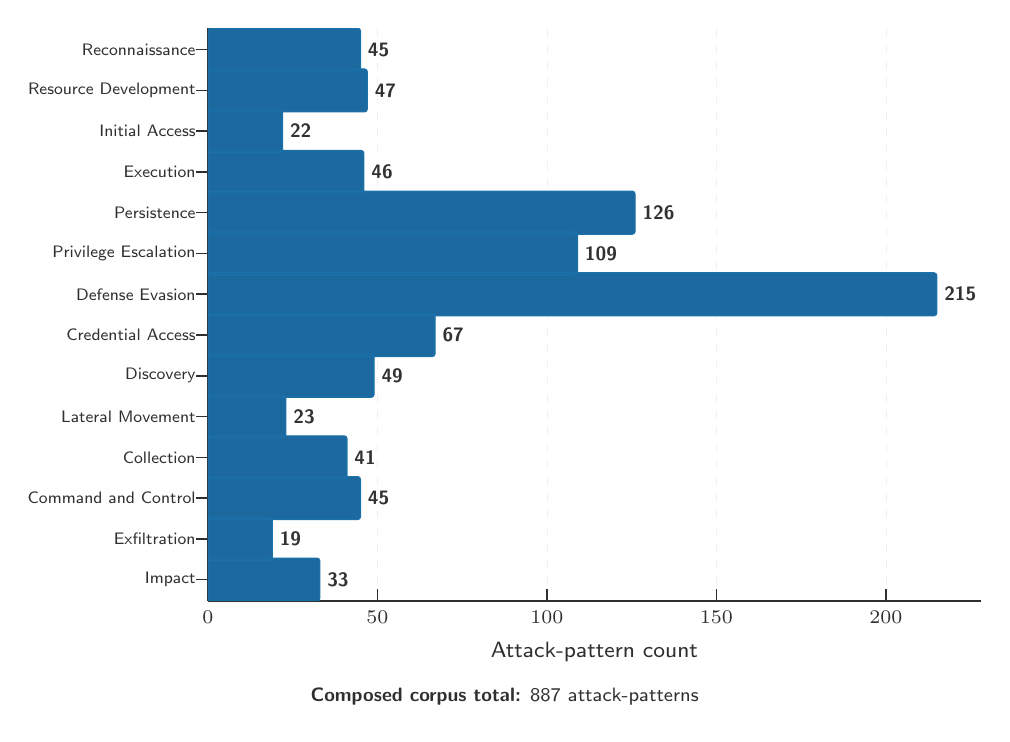
\begin{tikzpicture}
\begin{axis}[
  width=0.940\columnwidth,
  height=8.85cm,
  xbar,
  xmin=0, xmax=228,
  axis lines*=left,
  axis line style={draw=edgegray!92!black, line width=0.58pt},
  tick style={draw=edgegray!92!black, line width=0.55pt},
  xmajorgrids=true,
  grid style={dashgray!45, line width=0.28pt, dashed},
  y dir=reverse,
  ytick=data,
  yticklabels={
    Reconnaissance,
    Resource Development,
    Initial Access,
    Execution,
    Persistence,
    Privilege Escalation,
    Defense Evasion,
    Credential Access,
    Discovery,
    Lateral Movement,
    Collection,
    Command and Control,
    Exfiltration,
    Impact
  },
  yticklabel style={font=\sffamily\fontsize{6.0}{6.3}\selectfont, align=right,
                    inner xsep=0pt, text=edgegray!95!black},
  xtick={0,50,100,150,200},
  xticklabel style={font=\sffamily\fontsize{7.20}{7.55}\selectfont, text=edgegray!92!black},
  xlabel={Attack-pattern count},
  xlabel style={font=\sffamily\footnotesize, text=edgegray!92!black},
  enlarge y limits=0.04,
  bar width=5.45mm,
  nodes near coords,
  every node near coord/.append style={
    font=\sffamily\fontsize{6.8}{7.1}\selectfont\bfseries,
    text=edgegray!98!black,
    anchor=west,
    xshift=2.5pt,
    inner xsep=0pt,
    inner ysep=0pt
  },
  point meta=explicit symbolic
]
\addplot[
  draw=execblue!95!black,
  line width=0.42pt,
  fill=execblue!88!black,
  /tikz/rounded corners=1pt
] coordinates {
  (45,0)  [45]
  (47,1)  [47]
  (22,2)  [22]
  (46,3)  [46]
  (126,4) [126]
  (109,5) [109]
  (215,6) [215]
  (67,7)  [67]
  (49,8)  [49]
  (23,9)  [23]
  (41,10) [41]
  (45,11) [45]
  (19,12) [19]
  (33,13) [33]
};
\end{axis}
\node[
  font=\sffamily\scriptsize,
  text=edgegray!92!black,
  anchor=north,
  align=center
] at (current bounding box.south)
  [yshift=-0.09cm]
  {\textbf{Composed corpus total:} 887 attack-patterns};
\end{tikzpicture}%

  \caption{Technique count by MITRE \attack{} Enterprise tactic across the composed \stix{} dataset. Tactics are shown in the canonical Enterprise matrix order from Reconnaissance to Impact. For this ecosystem-level summary, each attack-pattern is assigned to one tactic bin, so the horizontal bars sum to 887 attack-pattern objects across all sources in the composed corpus. Quantitative analyses in this paper use only the \nAttackPatternObjects{} Enterprise attack-patterns with behavioral content (Section~\ref{sec:dataset}).}
  \Description{Horizontal bar chart of MITRE ATT\&CK Enterprise tactics in canonical matrix order from Reconnaissance to Impact, with bars showing attack-pattern counts in the composed STIX dataset. Each attack-pattern is placed into one tactic bin for visualization, so the bars sum to 887 attack-pattern objects across the composed corpus. The quantitative analyses use only the Enterprise subset with behavioral content.}
  \label{fig:full_chart}
\end{figure}

The analyst's role is limited to validating ordering, environmental assumptions, and parameter binding rather than inventing the behavioral scaffold from scratch. In our focal workflows, the dominant Stage~2 effort was binding missing parameters and checking SUT consistency. The end-to-end translation took on the order of one analyst-hour per workflow after Stage~1 had already produced the tactic-aligned scaffold. We report this only as a qualitative effort bound, not as a universal benchmark or an inter-analyst stability claim.


\subsection{Stage~3: Emulation Integration}
\label{sec:stage3}

Stage~3 converts the translated steps into an executable adversary representation. Any emulation environment capable of expressing actions, plans, and controlled execution can instantiate this stage. Each step becomes a platform-aware action with optional preconditions and postconditions. Ordered sets of actions form a behavioral plan that approximates a campaign or long-term threat operation, enabling consistency checks, assumption validation, and telemetry collection.

In this study, we instantiate Stage~3 using \caldera{}. Translated steps are mapped to abilities, adversary profiles, and operations. Abilities specify execution logic, expected output, and cleanup procedures; adversary profiles define the ordered set of abilities; and operations orchestrate execution, timing, agent assignment, and logging. Support scripts automate ability ingestion, profile construction, and repeated execution via the REST API. Once the human-curated steps are defined, all repetitive aspects of emulation are automated.

In our experiments, Stage~1 is instantiated with the \stix{}~2.1 Enterprise bundle, Stage~2 applies our translation procedure using \attack{} entries and structured CTI as authoritative sources, and Stage~3 maps the translated steps into \caldera{} artifacts. This separation keeps the methodology independent of any specific CTI format or emulation framework while enabling us to assess the limitations of available structured intelligence. Operationally, the methodology consumes structured CTI and a declared environment description, and it yields executable steps plus an explicit record of what the CTI did not provide.

To evaluate the methodology, we instantiate two case studies inspired by structured CTI, \emph{ShadowRay} and \emph{Soft Cell}. Their translated steps are analyzed in the legacy Docker-backed \caldera{} environment to test whether CTI-derived behavior can be enacted coherently once the missing procedure is made explicit. The result is not historical replay, but a controlled test of procedural completeness on a reproducible substrate.

Overall, the methodology provides a format-agnostic process for transforming descriptive structured CTI into a computable behavioral representation suitable for multi-host adversary emulation.

\section{Behavioral Analysis}
\label{sec:analysis}

Our analysis starts from two complementary views of the data. The first is the \emph{composed} \stix{} dataset, which aggregates multiple public CTI collections (including \mitre{} \attack{} Enterprise, CAPEC, DigitalSide, AlienVault OTX, and EclecticIQ). The second is the \mitre{} \attack{} Enterprise bundle itself, i.e., the official knowledge base maintained by \mitre{} for the Enterprise domain, serialized as \stix{}~2.x objects and periodically updated.

The distinction matters. \stix{} is a generic interchange format that defines object types and relationship structures for CTI. \attack{} is a behavioral knowledge base that organizes tactics, techniques, intrusion sets, campaigns, malware, and tools. The Enterprise bundle is one concrete \stix{} export of this knowledge base. The composed dataset broadens this export by incorporating additional \stix{} feeds that follow the same data model.

We first executed the whole processing pipeline on the composed dataset by parsing all bundles, deduplicating objects, constructing a typed graph, deriving campaign-technique vectors, and computing coverage, overlap, and clustering statistics across sources. The additional feeds increase breadth and redundancy by contributing more objects, including indicators and malware families. However, their campaign and intrusion-set descriptions are typically shorter and less structured than those found in \mitre{} \attack{} Enterprise.

For emulation purposes, the composed dataset and the Enterprise bundle share the same structural limitation: \stix{} does not define a dedicated procedure object with explicit ordering, preconditions, and environment bindings, and none of the sources in our corpus introduces such a construct as a custom extension. Consistent with prior work on CTI quality, we therefore find that most \stix{}-encoded artifacts remain sparse, incomplete, and procedurally underspecified. Campaign objects in particular rarely document the full incident, target environment, or execution prerequisites in machine-readable form.

The practical difference is one of degree rather than kind. Among the public feeds we parsed, the \attack{} Enterprise bundle still preserves the richest campaign-level structure, so we use it as the basis for the detailed behavioral analysis and clustering that follows. Each campaign is represented as a binary vector over Enterprise techniques, indicating which techniques appear at least once in that campaign. Intrusion sets are defined analogously from \stix{} \texttt{relationship} objects linking intrusion sets to \texttt{attack-pattern} or technique identifiers.

The Enterprise data contains more documented threat groups than publicly available campaigns. Each group is linked to one or more sets of techniques spanning phases such as Initial Access, Persistence, Privilege Escalation, Credential Access, Discovery, Lateral Movement, Command and Control, Collection, Exfiltration, and Impact. Together, these techniques form the group’s \emph{operational profile}, which is useful for connecting activity across campaigns, attributing incidents, and designing behavior-centered defenses.

We then compare campaigns with their corresponding intrusion sets to assess internal consistency in the Enterprise bundle. Because campaign entries are most informative when treated as technique sets, we examine how each campaign’s techniques relate to those attributed to its corresponding intrusion set. Both sides of the comparison come from the same Enterprise \stix{} representation used in the coverage and clustering analyses. We then manually cross-check a sample of these relationships against the \attack{} website.

By comparing the techniques observed in each campaign with those listed for the associated intrusion set, we find strong asymmetry in both directions. Across the 22 active campaign--intrusion-set attribution pairs with techniques on both sides, the median Jaccard overlap is only 10.0\%, and every pair covers less than half of the linked intrusion-set technique set. This is partly structural: intrusion sets aggregate behavior across multiple campaigns, whereas campaigns encode narrower operational slices. Even so, the relation is operationally weak because the linked intrusion-set profile often contributes much more behavior than the campaign itself documents.

A representative example is the \emph{Juicy Mix} campaign, which is linked to the \emph{OilRig} intrusion set: 64.3\% of the campaign's techniques appear in OilRig, but only 11.8\% of OilRig's documented techniques appear in Juicy Mix, as encoded in the Enterprise bundle. Our manual cross-checks against the \attack{} website revealed concrete cases in which the downloadable bundle and the website diverged on campaign--intrusion-set relationships. This shows that even frequently updated bundles can contain discrepancies in these links.

We do not attempt to model the exact source of these mismatches. For emulation, the practical implication is narrower: campaign-group mappings in the downloadable bundle should be treated as curated data that can diverge from the website and may therefore require spot checks in sensitive cases.

The composed dataset from Section~\ref{sec:dataset} broadens coverage across threat domains and allows cross-checks between providers~\cite{jin2024sharing}. It does not, however, add procedural depth: all sources rely on the same \stix{} object model, and none introduces structured fields for ordering, preconditions, or environment bindings beyond what the standard already provides. This is why the detailed quantitative analysis and emulation experiments use the Enterprise bundle: in our corpus, it preserves the most campaign-level structure even though it remains sparse and imperfect.

\begin{figure}[htpb]
\centering
% nocluster.tex — PCA scatter of 172 intrusion-set technique vectors
% AUTO-GENERATED by analyze_campaigns.py — DO NOT EDIT DATA BY HAND
% Points are REAL data from ATT&CK Enterprise v18.1, NOT synthetic.
% Design: white background, 4:3 aspect, single-color points to keep the
% takeaway focused on the absence of coherent clusters rather than on a
% secondary color-encoded variable.
% Host requirement: the parent document must load pgfplots (which loads TikZ).
\pgfplotsset{compat=1.18}%
\providecolor{execblue}{HTML}{1F77B4}%
\providecolor{ctired}{HTML}{D55E00}%
\providecolor{loopgreen}{HTML}{009E73}%
\providecolor{edgegray}{HTML}{333333}%
\providecolor{dashgray}{HTML}{D9DDE2}%
\providecolor{facegray}{HTML}{FFFFFF}%
\providecolor{midgray}{HTML}{666666}%
\providecolor{stagefill}{HTML}{F5F5F5}%
\providecommand{\silhouetteScore}{0.05}%
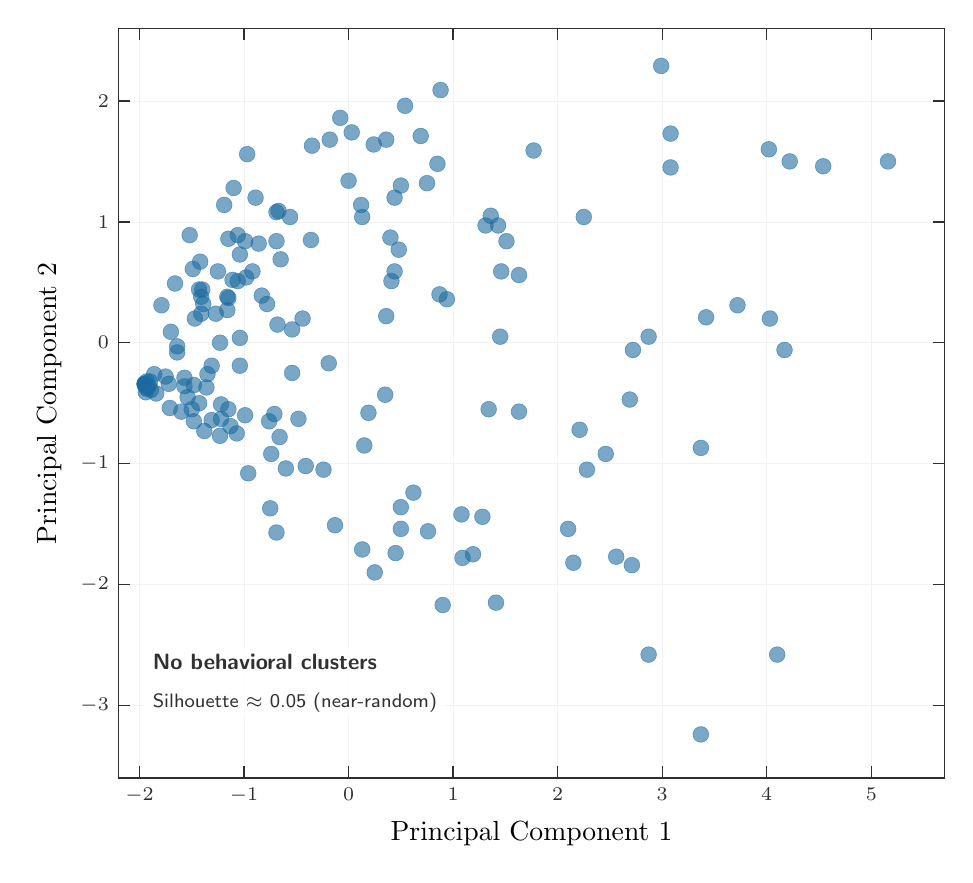
\begin{tikzpicture}
\begin{axis}[
  scale only axis,
  width  = 0.865\columnwidth,
  height = 0.785\columnwidth,
  xlabel = {Principal Component 1},
  ylabel = {Principal Component 2},
  xlabel style = {font=\sffamily\footnotesize, text=edgegray!92!black},
  ylabel style = {font=\sffamily\footnotesize, text=edgegray!92!black},
  xmin=-2.2, xmax=5.7,
  ymin=-3.6, ymax=2.6,
  tick label style = {font=\sffamily\scriptsize, text=edgegray!90!black},
  axis lines     = box,
  axis line style = {edgegray!92!black, line width=0.55pt},
  tick style     = {edgegray!92!black, line width=0.5pt, /pgfplots/minor tick length=1.5pt},
  xmajorgrids = true,
  ymajorgrids = true,
  grid style = {dashgray!38, line width=0.24pt},
  minor tick num = 0,
  axis background/.style={fill=facegray},
  only marks,
  mark         = *,
  mark size    = 2.85pt,
  mark options = {draw=execblue!95!black, fill=execblue!88!black, draw opacity=0.62, fill opacity=0.58, line width=0.20pt},
]
\addplot[only marks] coordinates {
(0.62,-1.24)[33]
(0.44,0.59)[28]
(2.56,-1.77)[57]
(3.37,-0.87)[64]
(-1.19,1.14)[9]
(3.08,1.45)[67]
(0.50,-1.54)[49]
(-0.60,-1.04)[22]
(-0.69,0.84)[11]
(2.46,-0.92)[56]
(4.03,0.20)[76]
(-1.93,-0.37)[4]
(1.41,-2.15)[41]
(4.54,1.46)[93]
(1.28,-1.44)[35]
(-0.44,0.20)[17]
(1.63,-0.57)[56]
(0.69,1.71)[34]
(0.00,1.34)[22]
(-0.68,0.15)[12]
(-0.92,0.59)[14]
(0.41,0.51)[31]
(-1.15,0.86)[12]
(1.63,0.56)[44]
(0.76,-1.56)[26]
(3.72,0.31)[79]
(-1.47,0.20)[6]
(2.87,0.05)[68]
(-1.48,-0.65)[5]
(1.09,-1.78)[48]
(1.34,-0.55)[40]
(0.87,0.40)[28]
(1.77,1.59)[41]
(3.42,0.21)[91]
(-1.23,-0.00)[9]
(-0.24,-1.05)[19]
(0.94,0.36)[36]
(0.12,1.14)[24]
(2.15,-1.82)[46]
(3.37,-3.24)[81]
(-0.76,-0.65)[17]
(4.17,-0.06)[79]
(1.46,0.59)[66]
(-1.10,1.28)[15]
(0.85,1.48)[34]
(-1.06,0.51)[12]
(1.08,-1.42)[44]
(2.72,-0.06)[53]
(3.08,1.73)[58]
(2.25,1.04)[56]
(-0.97,1.56)[14]
(4.22,1.50)[78]
(1.51,0.84)[40]
(-1.43,-0.50)[7]
(0.45,-1.74)[29]
(-0.66,-0.78)[15]
(5.16,1.50)[109]
(1.36,1.05)[50]
(0.36,0.22)[31]
(-1.43,0.44)[6]
(-0.75,-1.37)[17]
(4.02,1.60)[85]
(-0.69,-1.57)[43]
(2.87,-2.58)[59]
(0.54,1.96)[28]
(0.50,-1.36)[25]
(-0.69,1.08)[16]
(-1.49,0.61)[7]
(2.28,-1.05)[46]
(-0.41,-1.02)[42]
(1.31,0.97)[40]
(-1.11,0.52)[12]
(0.13,1.04)[21]
(-0.71,-0.59)[12]
(-0.35,1.63)[16]
(-0.19,-0.17)[16]
(-1.22,-0.63)[10]
(0.36,1.68)[29]
(-1.60,-0.57)[4]
(4.10,-2.58)[82]
(0.25,-1.90)[25]
(2.71,-1.84)[53]
(-1.57,-0.29)[4]
(-1.15,0.37)[11]
(1.19,-1.75)[31]
(-0.48,-0.63)[11]
(-1.31,-0.19)[6]
(1.45,0.05)[36]
(0.35,-0.43)[36]
(-1.64,-0.03)[5]
(-0.56,1.04)[18]
(0.90,-2.17)[64]
(-0.65,0.69)[19]
(-1.35,-0.26)[7]
(0.15,-0.85)[22]
(1.43,0.97)[41]
(-1.06,0.89)[12]
(0.75,1.32)[52]
(-0.36,0.85)[16]
(0.88,2.09)[30]
(0.24,1.64)[28]
(-1.79,0.31)[2]
(-0.18,1.68)[19]
(0.03,1.74)[19]
(2.10,-1.54)[49]
(2.69,-0.47)[57]
(-0.78,0.32)[15]
(2.99,2.29)[70]
(0.13,-1.71)[22]
(-0.74,-0.92)[27]
(-0.99,0.84)[9]
(0.44,1.20)[30]
(-0.86,0.82)[14]
(-1.38,-0.73)[14]
(-1.23,-0.77)[16]
(-0.83,0.39)[12]
(-1.16,0.38)[7]
(-1.66,0.49)[5]
(2.21,-0.72)[44]
(-1.64,-0.08)[4]
(-1.04,-0.19)[9]
(-1.42,0.67)[5]
(0.40,0.87)[29]
(0.19,-0.58)[23]
(-0.54,0.11)[14]
(-0.99,-0.60)[9]
(-1.52,0.89)[6]
(-0.89,1.20)[11]
(-0.96,-1.08)[11]
(0.48,0.77)[27]
(-0.67,1.09)[16]
(0.50,1.30)[31]
(-0.13,-1.51)[21]
(-1.31,-0.64)[9]
(-1.50,-0.55)[5]
(-1.16,0.27)[11]
(-1.54,-0.45)[5]
(-1.95,-0.34)[0]
(-1.39,0.32)[7]
(-1.04,0.04)[9]
(-1.36,-0.37)[13]
(-0.54,-0.25)[12]
(-1.15,-0.55)[9]
(-1.72,-0.34)[2]
(-1.07,-0.75)[10]
(-1.04,0.73)[9]
(-1.40,0.44)[7]
(-1.13,-0.69)[8]
(-0.08,1.86)[20]
(-1.41,0.24)[6]
(-1.48,-0.35)[8]
(-1.22,-0.51)[8]
(-0.98,0.54)[19]
(-1.57,-0.36)[4]
(-1.27,0.24)[11]
(-1.89,-0.39)[2]
(-1.41,0.38)[6]
(-1.71,-0.54)[2]
(-1.86,-0.26)[2]
(-1.84,-0.42)[3]
(-1.90,-0.32)[1]
(-1.25,0.59)[7]
(-1.75,-0.28)[4]
(-1.93,-0.38)[3]
(-1.94,-0.41)[2]
(-1.95,-0.35)[1]
(-1.70,0.09)[4]
(-1.91,-0.36)[1]
(-1.93,-0.32)[1]
(-1.95,-0.34)[0]
(-1.95,-0.34)[0]
(-1.95,-0.34)[0]
};
% --- Silhouette annotation (restrained, editorial) ---
\node[
  anchor=south west,
  inner xsep=3.2pt,
  inner ysep=2.0pt,
  align=left,
  text=edgegray!96!black,
  fill=white,
  fill opacity=0.90,
  text opacity=1
] at (rel axis cs:0.03,0.08)
  {{\sffamily\footnotesize\bfseries No behavioral clusters}\\[1.4pt]
   {\sffamily\scriptsize Silhouette $\approx$ \silhouetteScore{} (near-random)}};
\end{axis}
\end{tikzpicture}%

\caption{Technique-based similarity of \nIntrusionSets{} \mitre{} \attack{} Enterprise intrusion-sets.}
\Description{Technique-based similarity of \nIntrusionSets{} \mitre{} \attack{} Enterprise intrusion-sets.}
\label{fig:intrusionset}
\end{figure}

To better understand the behavioral structure encoded in Enterprise intrusion sets, we compute similarity from their technique vectors and apply principal component analysis (PCA), using the Jaccard distance as the similarity measure based on the presence or absence of the technique in the intrusion sets. Figure~\ref{fig:intrusionset} presents the resulting PCA. The projection forms a dense near-origin cloud without clearly separated families, suggesting that intrusion sets do not form coherent behavioral groupings. Instead, each intrusion set comprises a relatively small, idiosyncratic subset of techniques. Although intrusion sets cover more techniques than individual campaigns, they do not provide complete procedures. They usually do not capture relationships or the operational context among techniques. Therefore, while they are useful for high-level profiling, they are not adequate as standalone units for emulating adversaries without significant contextual reconstruction.

We also investigate whether common behavioral subsequences can be derived across campaigns. The operational assumption is simple: if Enterprise campaigns shared a stable technique backbone, a recurring subsequence should appear in tactic-ordered technique lists and could serve as a generic emulation template. For structural ordering, we use the canonical \attack{} tactic progression. This provides a consistent reconnaissance-to-impact scaffold without claiming that it reconstructs the chronology of any specific incident.

To quantify structural stability, we apply $k$-means clustering to the campaign-technique binary vectors and measure cohesion with the silhouette coefficient. We report $k=7$ because it yields an interpretable partition relative to the dominant tactic phases, not because we claim it is the statistically unique choice. Both the cluster assignment and the silhouette calculation use the same Euclidean geometry over these binary vectors. We use this consistently as a coarse structural probe, not as a claim that Euclidean distance is the only meaningful behavioral similarity notion.

At $k=7$, the mean silhouette score is \silhouetteScore{} (range $[-1, 1]$; values near zero indicate near-random assignment). As a baseline, we generate 1{,}000 random binary matrices with identical dimensions and sparsity and obtain a mean silhouette of $\silhouetteBaselineMean{} \pm \silhouetteBaselineStd{}$. A sensitivity sweep over $k \in [2,10]$ produces the same qualitative picture, with silhouettes remaining low throughout (`0.03`--`0.11`). A supplementary average-linkage agglomerative clustering run on Jaccard distances leaves the conclusion unchanged: silhouettes stay between 0.03 and 0.05 across the same $k$ range, including 0.03 at $k=7$. The real data therefore shows little reusable structure beyond chance. This directly refutes the operational assumption that campaign technique sets cluster into reusable behavioral families.

For sequence analysis, we compute the LCS between all $\binom{51}{2} = 1{,}275$ campaign pairs using the tactic-ordered technique lists. If campaigns shared a stable behavioral backbone, we would expect long common subsequences suitable as emulation templates. Instead, the mean LCS length is \lcsLengthMean{} techniques (median \lcsLengthMedian{}, max~\lcsLengthMax{}), and no pair shares more than a small fraction of its list with another. This conclusion is stable under tactic reassignment for multi-tactic techniques: across 200 randomized valid-tactic trials, the mean LCS remains between 2.727 and 2.760 and the median stays fixed at 2.0.

These results are consistent with the weak-cluster picture in Figure~\ref{fig:ccluster} and with prior studies that report sparsity, inconsistency, and incomplete behavioral specification in CTI sources~\cite{jin2024sharing,savat2021extractor,10117505}. Because the tactic-ordered lists are an organizational scaffold rather than a recovered timeline, the LCS results should be read as a descriptive probe of reusable structure, not as evidence about true chronological subsequences. Our negative result does not rely on this scaffold alone: the same picture already appears in unordered coverage, overlap, binary-vector clustering, and the order-free itemset probe in Appendix~\ref{app:itemset-probe}. In practice, the analysis reveals no robust common subsequence between campaigns and no universally shared pair of techniques.
Appendix~\ref{app:itemset-probe} reports a supplementary order-free probe with the same conclusion: even the most frequent five-technique itemset appears in only 6 of 51 campaigns (11.8\%).

\begin{figure}[htpb]
\centering
\resizebox{\columnwidth}{!}{% clusters.tex — Campaign cluster distribution (k=7, n=51)
% Proportional strip: compact single horizontal bar with proportional segments.
% Design: Okabe-Ito palette, standardized typography.
% Host requirement: the parent document must load TikZ.
\usetikzlibrary{decorations.pathreplacing}%
\providecolor{execblue}{HTML}{1F77B4}%
\providecolor{ctired}{HTML}{D55E00}%
\providecolor{loopgreen}{HTML}{009E73}%
\providecolor{midgray} {HTML}{666666}%
\providecolor{dashgray}{HTML}{D9DDE2}%
\providecolor{edgegray}{HTML}{333333}%
\providecolor{facegray}{HTML}{FFFFFF}%
\providecolor{stagefill}{HTML}{F5F5F5}%
\providecommand{\silhouetteScore}{0.05}%
\providecommand{\silhouetteBaselineMean}{-0.01}%
\providecommand{\silhouetteBaselineStd}{0.01}%
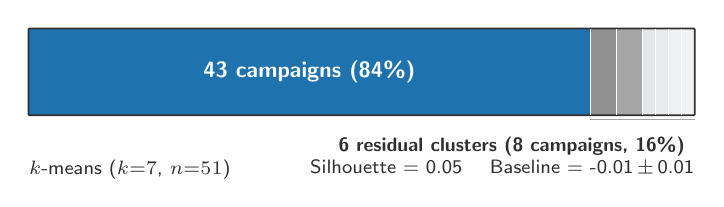
\begin{tikzpicture}[font=\sffamily]

\def\W{8.46}       % total strip width (cm) — exact ACM columnwidth
\def\H{1.10}       % strip height (cm) — matched to Figure 5 for visual consistency
\def\N{51}          % total campaigns

% Cluster sizes (sorted descending)
% C1=43, C2=2, C3=2, C4=1, C5=1, C6=1, C7=1

% Proportional widths
\pgfmathsetmacro{\wA}{43/\N*\W}    % dominant
\pgfmathsetmacro{\wB}{2/\N*\W}     % size-2 cluster
\pgfmathsetmacro{\wC}{1/\N*\W}     % singleton

% --- Segments (left to right: dominant, 2×size-2, 4×singletons) ---
\def\cx{0}

% C1 — dominant (43) — paper's primary data color
\fill[execblue!96!black, rounded corners=0.3pt]
  (\cx,0) rectangle (\wA,\H);
\node[white, font=\sffamily\bfseries\fontsize{7.8}{8.2}\selectfont, align=center]
  at (\wA/2, \H/2) {43 campaigns (84\%)};
\pgfmathsetmacro{\cx}{\wA}

% C2 — size 2 — muted grays (residual)
\fill[midgray!72] (\cx,0) rectangle ({\cx+\wB},\H);
\pgfmathsetmacro{\cx}{\cx+\wB}

% C3 — size 2 — slightly lighter
\fill[midgray!58] (\cx,0) rectangle ({\cx+\wB},\H);
\pgfmathsetmacro{\cx}{\cx+\wB}

% C4–C7 — singletons — progressively lighter
\fill[dashgray!72]  (\cx,0) rectangle ({\cx+\wC},\H);
\pgfmathsetmacro{\cx}{\cx+\wC}
\fill[dashgray!58]  (\cx,0) rectangle ({\cx+\wC},\H);
\pgfmathsetmacro{\cx}{\cx+\wC}
\fill[dashgray!45]  (\cx,0) rectangle ({\cx+\wC},\H);
\pgfmathsetmacro{\cx}{\cx+\wC}
\fill[dashgray!34]  (\cx,0) rectangle ({\cx+\wC},\H);

% --- Outline ---
\draw[edgegray!92!black, line width=0.64pt, rounded corners=0.3pt] (0,0) rectangle (\W,\H);

% --- Thin dividers between residual segments ---
\pgfmathsetmacro{\dA}{\wA}
\pgfmathsetmacro{\dB}{\wA+\wB}
\pgfmathsetmacro{\dC}{\wA+2*\wB}
\pgfmathsetmacro{\dD}{\wA+2*\wB+\wC}
\pgfmathsetmacro{\dE}{\wA+2*\wB+2*\wC}
\pgfmathsetmacro{\dF}{\wA+2*\wB+3*\wC}
\foreach \x in {\dA,\dB,\dC,\dD,\dE,\dF}{
  \draw[white, line width=0.42pt] (\x,0) -- (\x,\H);
}

% --- Residual annotation (below strip, right-aligned under residual area) ---
\pgfmathsetmacro{\residStart}{\wA}
\pgfmathsetmacro{\residEnd}{\W}
\pgfmathsetmacro{\residMid}{(\residStart+\residEnd)/2}

% Residual marker under strip
\draw[edgegray!44, line width=0.42pt]
  (\residStart, -0.06) -- (\residEnd, -0.06);
\node[
  font=\sffamily\fontsize{7.10}{7.40}\selectfont\bfseries,
  text=edgegray!92!black,
  anchor=north east,
  align=right
]
  at (\W, -0.15)
  {6 residual clusters (8 campaigns, 16\%)};

% --- Footer with metrics ---
\node[
  font=\sffamily\fontsize{7.10}{7.40}\selectfont,
  text=edgegray!92!black,
  anchor=north west,
  align=left,
  inner xsep=0pt,
  inner ysep=0pt
]
  at (0, -0.56)
  {$k$-means ($k{=}7$, $n{=}51$)};

\node[
  font=\sffamily\fontsize{7.10}{7.40}\selectfont,
  text=edgegray!92!black,
  anchor=north east,
  align=right,
  inner xsep=0pt,
  inner ysep=0pt
]
  at (\W, -0.56)
  {Silhouette = \silhouetteScore{} \quad Baseline = \silhouetteBaselineMean{}\,$\pm$\,\silhouetteBaselineStd{}};

\end{tikzpicture}%
}
\caption{Campaign cluster sizes induced by $k$-means over technique-overlap vectors. The area chart shows how 51 Enterprise campaigns are partitioned when clustered with $k=7$, highlighting one dominant cluster and several tiny residual clusters rather than well-separated behavioral families.}
\Description{Single horizontal proportional strip showing the sizes of seven clusters produced by k-means on ATT\&CK Enterprise campaign-technique vectors. One dominant cluster contains 43 campaigns, two residual clusters contain 2 campaigns each, and four residual clusters are singletons, indicating weak structure.}
\label{fig:ccluster}
\end{figure}

A common operational assumption is that APT campaigns share a stable behavioral backbone suitable for generating generic emulation profiles. Our analysis of the 51 Enterprise campaigns contradicts this view. Campaign coverage is sparse: only \campaignCoveragePct\% of all Enterprise techniques appear in at least one campaign, leaving \campaignCoverageUnusedPct\% unused in any campaign instance (Figure~\ref{fig:coverage}).

No technique is universal, and even the most frequent ones are far from ubiquitous. The most frequent technique, \texttt{\topTechniqueId} (\topTechniqueLabel), appears in \topTechniqueInCampaigns{} campaigns (\topTechniquePct\%). No single technique appears in every campaign, and no pair of techniques co-occurs universally. The long-tailed frequency distribution and low-cohesion clusters together indicate that campaigns are idiosyncratic. A small number of behaviors, such as \texttt{T1105}, \texttt{T1588.002}, and \texttt{T1071.001}, appear in many campaigns, while most techniques are rarely used.

At the same time, narrowness does not imply indistinguishability. Using positive-evidence identifiability over the current Enterprise campaign-technique profiles, we find that all 51 campaigns are distinguishable from the others by some subset of their own techniques, and every campaign admits a distinguishing witness of size at most three. Formally, a witness for campaign $C$ is a subset of techniques in $C$ that is not contained in any other campaign profile; we compute the minimum witness exactly over the reduced campaign-difference sets.

This is a structural result about profile separability, not a claim about attribution in the wild or about procedural completeness. Under the same model, 145 of 168 intrusion-set profiles are distinguishable, while 23 are subsumed by larger profiles and admit no positive witness. Campaign objects can therefore be distinctive as sparse behavioral slices while still remaining too underspecified to execute directly.

\begin{figure}[htpb]
\centering
\resizebox{\columnwidth}{!}{% venn-techniques.tex — Partition of ATT&CK techniques across campaign and intrusion-set usage
% Redesigned from Venn to proportional overlap partition for stricter semantics.
% Host requirement: the parent document must load TikZ.
\usetikzlibrary{calc,decorations.pathreplacing}%
\providecolor{execblue}{HTML}{1F77B4}%
\providecolor{ctired}{HTML}{D55E00}%
\providecolor{loopgreen}{HTML}{009E73}%
\providecolor{edgegray}{HTML}{333333}%
\providecolor{midgray}{HTML}{666666}%
\providecolor{dashgray}{HTML}{D9DDE2}%
\providecolor{facegray}{HTML}{FFFFFF}%
\providecolor{stagefill}{HTML}{F5F5F5}%
\providecommand{\nTechniquesAnalysis}{691}%
\providecommand{\campaignTechniqueCount}{297}%
\providecommand{\campaignCoveragePct}{43.0}%
\providecommand{\intrusionSetTechniqueCount}{488}%
\providecommand{\intrusionSetCoveragePct}{70.6}%
\providecommand{\campaignOnlyCount}{29}%
\providecommand{\campaignOnlyPct}{4.2}%
\providecommand{\sharedTechniqueCount}{268}%
\providecommand{\sharedPct}{38.8}%
\providecommand{\intrusionSetOnlyCount}{220}%
\providecommand{\intrusionSetOnlyPct}{31.8}%
\providecommand{\unusedTechniqueCount}{174}%
\providecommand{\unusedPct}{25.2}%
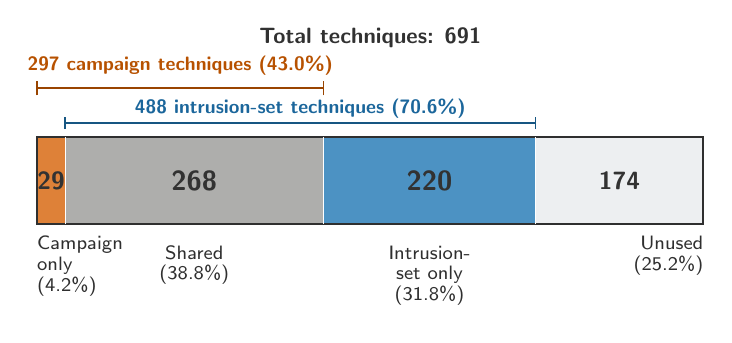
\begin{tikzpicture}[font=\sffamily, every node/.style={outer sep=0pt}]

\def\W{8.46}
\def\H{1.10}
\def\N{691}

\pgfmathsetmacro{\wCampaignOnly}{\campaignOnlyCount/\N*\W}
\pgfmathsetmacro{\wShared}{\sharedTechniqueCount/\N*\W}
\pgfmathsetmacro{\wIntrOnly}{\intrusionSetOnlyCount/\N*\W}
\pgfmathsetmacro{\wUnused}{\unusedTechniqueCount/\N*\W}

\pgfmathsetmacro{\xA}{0}
\pgfmathsetmacro{\xB}{\wCampaignOnly}
\pgfmathsetmacro{\xC}{\wCampaignOnly+\wShared}
\pgfmathsetmacro{\xD}{\wCampaignOnly+\wShared+\wIntrOnly}
\pgfmathsetmacro{\xE}{\W}

% Main partition bar
\fill[ctired!78!white] (\xA,0) rectangle (\xB,\H);
\fill[ctired!42!execblue!55!white] (\xB,0) rectangle (\xC,\H);
\fill[execblue!80!white] (\xC,0) rectangle (\xD,\H);
\fill[dashgray!48] (\xD,0) rectangle (\xE,\H);
\draw[edgegray!92!black, line width=0.64pt] (\xA,0) rectangle (\xE,\H);
\foreach \x in {\xB,\xC,\xD}{
  \draw[white, line width=0.42pt] (\x,0) -- (\x,\H);
}

% Top total label
\node[
  font=\sffamily\bfseries\fontsize{7.9}{8.3}\selectfont,
  text=edgegray!96!black,
  anchor=south,
  inner sep=0pt
] at ({\W/2},\H+1.14) {Total techniques: \nTechniquesAnalysis};

% Campaign span
\draw[ctired!72!black, line width=0.70pt]
  (\xA,\H+0.62) -- (\xC,\H+0.62);
\draw[ctired!72!black, line width=0.50pt] (\xA,\H+0.53) -- (\xA,\H+0.71);
\draw[ctired!72!black, line width=0.50pt] (\xC,\H+0.53) -- (\xC,\H+0.71);
\node[
  font=\sffamily\fontsize{7.10}{7.45}\selectfont\bfseries,
  text=ctired!86!black,
  anchor=south,
  align=center,
  inner sep=0pt
] at ({(\xA+\xC)/2},\H+0.78)
  {\campaignTechniqueCount\ campaign techniques (\campaignCoveragePct\%)};

% Intrusion-set span
\draw[execblue!72!black, line width=0.70pt]
  (\xB,\H+0.18) -- (\xD,\H+0.18);
\draw[execblue!72!black, line width=0.50pt] (\xB,\H+0.10) -- (\xB,\H+0.26);
\draw[execblue!72!black, line width=0.50pt] (\xD,\H+0.10) -- (\xD,\H+0.26);
\node[
  font=\sffamily\fontsize{7.10}{7.45}\selectfont\bfseries,
  text=execblue!86!black,
  anchor=south,
  align=center,
  inner sep=0pt,
  text width=4.90cm
] at ({(\xB+\xD)/2},\H+0.24)
  {\intrusionSetTechniqueCount\ intrusion-set techniques (\intrusionSetCoveragePct\%)};

% Counts inside segments
\node[font=\sffamily\bfseries\fontsize{8.6}{8.9}\selectfont, text=edgegray!98!black]
  at ({(\xA+\xB)/2},0.49*\H) {\campaignOnlyCount};
\node[font=\sffamily\bfseries\fontsize{9.8}{10.2}\selectfont, text=edgegray!98!black]
  at ({(\xB+\xC)/2},0.49*\H) {\sharedTechniqueCount};
\node[font=\sffamily\bfseries\fontsize{9.8}{10.2}\selectfont, text=edgegray!98!black]
  at ({(\xC+\xD)/2},0.49*\H) {\intrusionSetOnlyCount};
\node[font=\sffamily\bfseries\fontsize{8.6}{8.9}\selectfont, text=edgegray!98!black]
  at ({(\xD+\xE)/2},0.49*\H) {\unusedTechniqueCount};

% Segment labels
\node[
  font=\sffamily\fontsize{7.15}{7.55}\selectfont,
  text=edgegray!92!black,
  align=left,
  text width=1.30cm,
  anchor=north west,
  inner sep=0pt
] at (\xA,-0.16) {Campaign only\\(\campaignOnlyPct\%)};
\node[
  font=\sffamily\fontsize{7.15}{7.55}\selectfont,
  text=edgegray!92!black,
  align=center,
  text width=0.96cm,
  anchor=north
] at ({(\xB+\xC)/2},-0.16) {Shared\\(\sharedPct\%)};
\node[
  font=\sffamily\fontsize{7.15}{7.55}\selectfont,
  text=edgegray!92!black,
  align=center,
  text width=1.78cm,
  anchor=north
] at ({(\xC+\xD)/2},-0.16) {Intrusion-set only\\(\intrusionSetOnlyPct\%)};
\node[
  font=\sffamily\fontsize{7.15}{7.55}\selectfont,
  text=edgegray!92!black,
  align=right,
  text width=1.05cm,
  anchor=north east,
  inner sep=0pt
] at (\xE,-0.16) {Unused\\(\unusedPct\%)};

\end{tikzpicture}%
}
\caption{Technique usage across 51 \mitre{} \attack{} Enterprise campaigns and \nIntrusionSets{} intrusion sets.}
\Description{Partition bar showing the \nTechniquesAnalysis{} Enterprise techniques split into campaign-only, shared, intrusion-set-only, and unused segments. Spans above the bar indicate that campaigns cover \campaignTechniqueCount{} techniques (\campaignCoveragePct\%) while intrusion sets cover \intrusionSetTechniqueCount{} techniques (\intrusionSetCoveragePct\%).}
\label{fig:coverage}
\end{figure}

These results are consistent with prior studies that report structural variability, sparse field usage, and difficulty extracting actionable temporal structure from public CTI~\cite{jin2024sharing,savat2021extractor,10117505}. Our contribution is to connect those well-known data-quality problems directly to the emulation setting: publicly available CTI may still distinguish behaviors, but it does not expose the regular procedural structure needed to derive reusable execution templates.

The main findings are synthesized as follows:

\noindent
\begin{textbox}
  \textbf{Campaign heterogeneity:}
  Enterprise campaigns employ sparse technique subsets: no single technique is universal, and clustering/LCS analyses reveal no common behavioral backbone across campaigns.

  \textbf{Technique dispersion:}
  Only \campaignCoveragePct\% of \mitre{} \attack{} Enterprise techniques appear in any campaign (Fig.~\ref{fig:coverage}), yielding a long-tailed frequency distribution with no dominant core of shared behavior.

  \textbf{Positive-evidence identifiability:}
  Despite this sparsity, all 51 campaign profiles are distinguishable within the Enterprise corpus by small positive witnesses, with all campaigns separable by at most three techniques. Under the same model, 145 of 168 intrusion-set profiles are distinguishable, while 23 are subsumed by larger profiles. Distinguishability in profile space therefore does not imply executability.

  \textbf{Intrusion-set coverage:}
  Intrusion sets account for \intrusionSetCoveragePct\% of Enterprise techniques and preserve broader, less fragmented behavioral profiles than individual campaign objects.

  \textbf{Structural asymmetry:}
  Across 51 campaigns, 297 techniques are used, and 29 of them do not appear in the corresponding intrusion-set profiles. Intrusion sets, by contrast, use 488 techniques, including 220 that appear in no campaign. This asymmetry shows that campaigns encode narrow episodic slices of activity, while intrusion sets span a broader behavioral space.

  \textbf{Broken campaign-group mapping:}
  Several campaigns are linked to intrusion sets with limited technique overlap, and some campaign technique sets contradict their group-level profiles, reflecting inconsistencies between website and Enterprise bundle relationships (e.g., Juicy Mix vs.\ OilRig).

  \textbf{IOC role:}
  Although IoCs are not the focus of our quantitative analysis, our findings align with prior work that treats indicators primarily as short-lived signals for triage and hunting, rather than as sufficient input for reconstructing multi-step adversary behavior or for robust attribution.

  \textbf{Modeling implication:}
  For adversary emulation, intrusion-set-centric modeling preserves more behavioral coverage than campaign-centric approaches, and current \stix{}-encoded campaigns should be treated as partial behavioral hints rather than procedural templates.
\end{textbox}

\section{Emulation Setup}
\label{sec:emulation}

In Stage~1, the relevant intrusion sets, campaigns, and techniques are loaded directly from the \stix{} bundle and ordered with the conservative tactic scaffold introduced earlier. Stage~2 then refines those abstractions into runnable commands through analyst validation rather than historical reconstruction.

In this study, Stage~3 uses \caldera{}~5.3.0 strictly as an execution engine. \caldera{} does not interpret \stix{} objects, infer sequencing, or supply missing parameters. Each translated technique therefore becomes an explicit \caldera{} ability with one command and, when appropriate, cleanup logic; the resulting abilities are arranged into adversary profiles using the Stage~1 scaffold. When a step fails, the failure points to a missing assumption, parameter, or precondition in the CTI-derived representation rather than to framework-side inference.

Experiments were conducted in a fully isolated containerized testbed built from the legacy Docker artifact, a frozen package of eight curated adversary workflows plus shared attacker/target service definitions, with a \caldera{} server, an attacker-side Kali agent, and target-side services connected through private Docker networks. In this setup, \caldera{} functions as the emulation orchestrator and the Kali agent serves as the execution agent, consistent with the conceptual components in Figure~\ref{fig:env}. The environment is not intended to approximate a real victim infrastructure. Its role is to provide a stable substrate for testing whether CTI-derived steps can be enacted without contradiction.

Concretely, the audited substrate is composed of four containers connected through three private Docker networks: a \caldera{} server, a Kali execution node, an exposed Nginx service, and an internal database service. We report this topology only to bound reproducibility of the shared laboratory base, not to claim that the environment reconstructs the historical victim networks behind the focal campaigns.

Operationally, each enactment experiment requires four elements: a substrate to run on, the campaign-relevant weaknesses or exposed services that make the steps executable, a translated workflow, and observable execution traces. Importantly, the legacy artifact preloads campaign-specific target bootstrap scripts into one shared laboratory substrate rather than provisioning a fresh per-campaign SUT. As a consequence, even campaigns that historically involved multiple hosts, such as Soft Cell, are evaluated here as procedural enactments over a common controlled environment. Any observed progress or blocking point must be interpreted in that context.

\begin{figure}[t]
    \centering
\resizebox{\columnwidth}{!}{% environment.tex — execution environment for CTI-derived behaviors
% Design goal: austere single-column architecture diagram with horizontally
% aligned attacker and target panels sharing the same visual centerline.
% Host requirement: the parent document must load TikZ.
\usetikzlibrary{arrows.meta,calc}%
\providecolor{execblue}{HTML}{1F77B4}%
\providecolor{ctired}{HTML}{D55E00}%
\providecolor{loopgreen}{HTML}{009E73}%
\providecolor{midgray}{HTML}{666666}%
\providecolor{dashgray}{HTML}{D9DDE2}%
\providecolor{edgegray}{HTML}{333333}%
\providecolor{facegray}{HTML}{FFFFFF}%
\providecolor{stagefill}{HTML}{F5F5F5}%
\tikzset{
  pics/computer/.style={
    code={
      \draw[draw=edgegray!62, fill=white, line width=0.56pt, rounded corners=1.5pt]
        (-0.33,0.20) rectangle (0.33,-0.10);
      \draw[draw=edgegray!28, fill=edgegray!2, line width=0.36pt, rounded corners=0.8pt]
        (-0.25,0.13) rectangle (0.25,-0.03);
      \draw[edgegray!50, line width=0.38pt] (0,-0.10) -- (0,-0.21);
      \draw[edgegray!50, line width=0.38pt] (-0.14,-0.23) -- (0.14,-0.23);
    }
  },
  pics/computer-faded/.style={
    code={
      \draw[draw=edgegray!34, fill=edgegray!2, line width=0.50pt, rounded corners=1.5pt]
        (-0.33,0.20) rectangle (0.33,-0.10);
      \draw[draw=edgegray!20, fill=edgegray!1, line width=0.34pt, rounded corners=0.8pt]
        (-0.25,0.13) rectangle (0.25,-0.03);
      \draw[edgegray!28, line width=0.36pt] (0,-0.10) -- (0,-0.21);
      \draw[edgegray!28, line width=0.36pt] (-0.14,-0.23) -- (0.14,-0.23);
    }
  }
}%
\begin{tikzpicture}[
  x=1cm,y=1cm,
  font=\sffamily,
  line cap=round,
  line join=round,
  panel/.style={
    draw=edgegray!54,
    rounded corners=5.2pt,
    line width=0.88pt,
    fill=white
  },
  titlelabel/.style={
    font=\sffamily\bfseries\fontsize{8.4}{8.8}\selectfont,
    text=edgegray!96!black
  },
  sublabel/.style={
    font=\sffamily\fontsize{7.0}{7.3}\selectfont,
    text=edgegray!78!black
  },
  sutlabel/.style={
    font=\sffamily\bfseries\fontsize{7.30}{7.65}\selectfont,
    text=execblue!86!black
  },
  machine/.style={
    rounded corners=4.2pt,
    line width=0.88pt,
    minimum width=1.92cm,
    minimum height=0.84cm,
    align=center,
    inner sep=3pt,
    font=\sffamily\bfseries\fontsize{7.20}{7.55}\selectfont
  },
  orchestrator/.style={machine, draw=execblue!78!black, fill=execblue!6, text=execblue!92!black},
  agent/.style={machine, draw=execblue!52!black, fill=execblue!3, text=edgegray!96!black},
  c2loop/.style={
    -{Latex[length=5.0pt,width=4.0pt]},
    line width=1.18pt,
    draw=loopgreen!90!black
  },
  attackarrow/.style={
    -{Latex[length=5.4pt,width=4.2pt]},
    line width=1.18pt,
    draw=ctired!90!black
  },
  exposurebox/.style={
    draw=ctired!72!black,
    fill=ctired!5,
    rounded corners=4.6pt,
    line width=0.96pt
  },
  sutbox/.style={
    draw=execblue!50!black,
    fill=execblue!4,
    rounded corners=4.6pt,
    line width=0.84pt
  },
  hostlabel/.style={
    font=\sffamily\fontsize{6.8}{7.1}\selectfont\bfseries,
    text=edgegray!94!black,
    inner sep=0pt,
    anchor=north
  },
  hostlabelfaded/.style={
    font=\sffamily\fontsize{6.8}{7.1}\selectfont\bfseries,
    text=edgegray!68!black,
    inner sep=0pt,
    anchor=north
  }
]

\def\LeftW{2.72}
\def\Gap{0.26}
\def\RightW{5.92}
\def\PanelH{3.48}
\def\CenterY{-0.12}
\def\HostSep{1.18}

% --- Panel frames ---------------------------------------------------------
\node[panel, minimum width=\LeftW cm, minimum height=\PanelH cm, anchor=center] (leftpanel) at ({\LeftW/2},\CenterY) {};
\node[panel, minimum width=\RightW cm, minimum height=\PanelH cm, anchor=center] (rightpanel) at ({\LeftW+\Gap+\RightW/2},\CenterY) {};

\coordinate (titlebase) at ($(leftpanel.north)+(0,0.14)$);
\node[titlelabel, anchor=base] at (titlebase) {Attacker Infrastructure};
\node[titlelabel, anchor=base] at ($(rightpanel.center |- titlebase)$) {Target Environment};
\node[
  sublabel,
  inner xsep=0pt,
  inner ysep=0pt,
  anchor=north
] at ($(rightpanel.north)+(0,-0.22)$) {shared laboratory substrate};

% --- Left panel content ---------------------------------------------------
\node[orchestrator] (orch) at ($(leftpanel.center)+(0,0.68)$) {Emulation\\Orchestrator};
\node[agent]        (agnt) at ($(leftpanel.center)+(0,-0.74)$) {Execution\\Agent};

\coordinate (calLeft)  at ($(orch.west)!0.50!(orch.south west)$);
\coordinate (calRight) at ($(orch.east)!0.50!(orch.south east)$);
\coordinate (agLeft)   at ($(agnt.west)!0.50!(agnt.north west)$);
\coordinate (agRight)  at ($(agnt.east)!0.50!(agnt.north east)$);

\draw[c2loop]
  (agLeft) .. controls ($(agLeft)+(-0.38,0.18)$) and ($(calLeft)+(-0.38,-0.18)$) .. (calLeft);
\draw[c2loop]
  (calRight) .. controls ($(calRight)+(0.38,-0.18)$) and ($(agRight)+(0.38,0.18)$) .. (agRight);

\node[
  font=\sffamily\bfseries\fontsize{7.20}{7.55}\selectfont,
  text=loopgreen!82!black,
  fill=white,
  inner xsep=3.6pt,
  inner ysep=1.1pt,
  rounded corners=3pt
] at ($(orch)!0.5!(agnt)$) {C2};

% --- Right panel content --------------------------------------------------
\node[sutbox, minimum width=5.56cm, minimum height=2.32cm, anchor=center] (sut)
  at ($(rightpanel.center)+(0,-0.18)$) {};
\coordinate (h1) at ($(sut.west)+(1.10,0.00)$);
\coordinate (h2) at ($(h1)+(\HostSep,0)$);
\coordinate (h3) at ($(h2)+(\HostSep,0)$);
\coordinate (hN) at ($(sut.east)+(-0.50,0.00)$);
\coordinate (hd) at ($($(h3)+(0.36,0)$)!0.5!($(hN)+(-0.36,0)$)$);

\node[exposurebox, minimum width=3.98cm, minimum height=1.26cm, anchor=center] (expBand)
  at ($(h1)!0.5!(h3)$) {};

\coordinate (kaliAttack) at (agnt.east);
\coordinate (attackLead) at ($(kaliAttack)+(0.34,0)$);
\coordinate (attackJoin) at ($(expBand.west)+(0.18,0.03)$);
\coordinate (attackEnd) at ($(h1)+(-0.38,0.03)$);
\draw[draw=ctired!90!black, line width=1.18pt]
  (kaliAttack) -- (attackLead)
    .. controls ($(attackLead)+(0.94,0)$)
    and ($(attackJoin)+(-1.08,0)$)
    .. (attackJoin);
\draw[attackarrow] (attackJoin) -- (attackEnd);
\draw[attackarrow] ($(h1)+(0.36,0)$) -- ($(h2)+(-0.36,0)$);
\draw[attackarrow] ($(h2)+(0.36,0)$) -- ($(h3)+(-0.36,0)$);
\draw[draw=ctired!72!black, line width=0.94pt, dash pattern=on 2.2pt off 1.8pt]
  ($(h3)+(0.34,0)$) -- ($(hN)+(-0.06,0)$);

\pic[scale=1.10] at (h1) {computer};
\pic[scale=1.10] at (h2) {computer};
\pic[scale=1.10] at (h3) {computer};
\pic[scale=1.10] at (hN) {computer-faded};

\node[
  sutlabel,
  fill=white,
  inner xsep=1.8pt,
  inner ysep=0.8pt,
  rounded corners=1.8pt,
  anchor=north west
] at ($(sut.north west)+(0.22,-0.16)$) {system under test (SUT)};

\node[
  font=\sffamily\bfseries\fontsize{7.20}{7.55}\selectfont,
  text=ctired!90!black,
  anchor=north
] at ($(expBand.south)+(0,-0.06)$) {campaign-relevant exposure};

\node[hostlabel] at ($(h1)+(0,-0.33)$) {Host 1};
\node[hostlabel] at ($(h2)+(0,-0.33)$) {Host 2};
\node[hostlabel] at ($(h3)+(0,-0.33)$) {Host 3};
\node[hostlabelfaded, text=edgegray!88!black] at ($(hd)+(0,-0.39)$) {\textbullet\kern2pt\textbullet\kern2pt\textbullet};
\node[hostlabelfaded] at ($(hN)+(0,-0.33)$) {Host $N$};

\end{tikzpicture}%
}
    \caption{Isolated environment used for executing CTI-derived behaviors. The left panel shows the attacker infrastructure, composed of the \caldera{} orchestrator and a Kali execution agent linked by a command-and-control loop; the right panel shows the shared laboratory substrate, containing a declared system under test (SUT), with the campaign-relevant exposure highlighted across one or more target hosts.}
    \Description{Single-column diagram with the attacker infrastructure in the left panel and the target environment in the right panel. The left panel contains a Caldera orchestrator and a Kali execution agent connected by a command-and-control loop. The right panel contains a shared laboratory substrate, an inner system-under-test box, and a highlighted campaign-relevant exposure region spanning multiple target hosts.}
    \label{fig:env}
\end{figure}

\begin{figure*}[htpb]
    \centering
    \resizebox{\textwidth}{!}{% gap-example.tex — Concrete illustration of the procedural semantics gap
% Design goal: wide, austere, structurally aligned two-panel comparison.
% Host requirement: the parent document must load TikZ.
\usetikzlibrary{arrows.meta,calc,positioning,shapes.geometric}%
\providecolor{execblue}{HTML}{1F77B4}%
\providecolor{ctired}{HTML}{D55E00}%
\providecolor{loopgreen}{HTML}{009E73}%
\providecolor{midgray}{HTML}{666666}%
\providecolor{dashgray}{HTML}{D9DDE2}%
\providecolor{edgegray}{HTML}{333333}%
\providecolor{facegray}{HTML}{FFFFFF}%
\providecolor{stagefill}{HTML}{F5F5F5}%
\providecommand{\gapkey}[1]{{\sffamily\fontsize{7.20}{7.55}\selectfont\textcolor{midgray!90!black}{#1}}}%
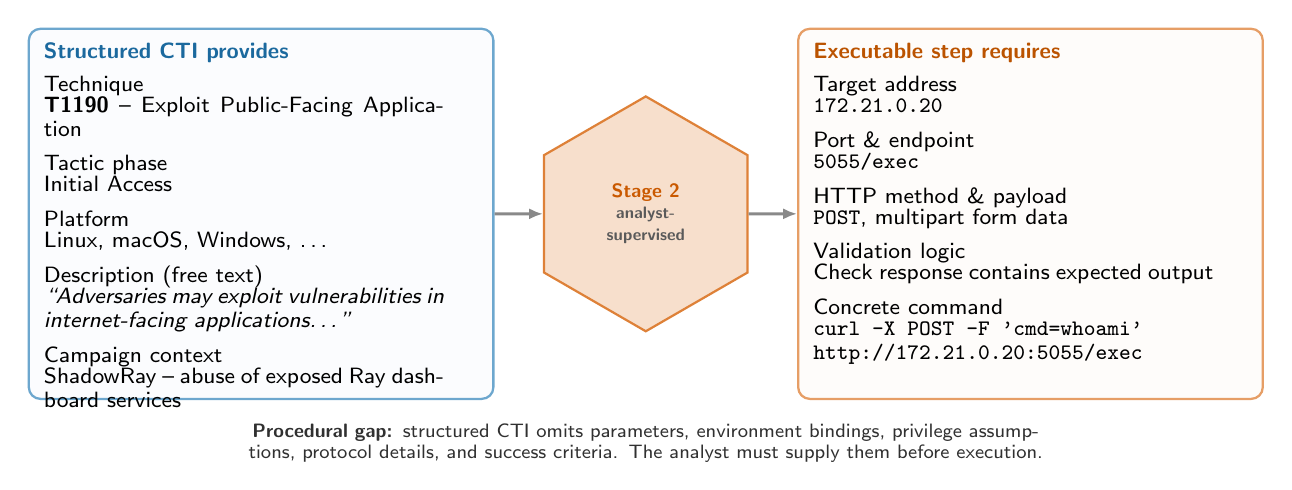
\begin{tikzpicture}[
  font=\sffamily,
  panel/.style={
    rounded corners=4.2pt,
    line width=0.82pt,
    minimum width=\PanelW,
    minimum height=\PanelH,
    fill=white
  },
  stixpanel/.style={panel, draw=execblue!65, fill=execblue!2},
  execpanel/.style={panel, draw=ctired!60, fill=ctired!2},
  bridgehex/.style={
    shape=regular polygon,
    regular polygon sides=6,
    shape border rotate=30,
    minimum size=2.16cm,
    text width=1.70cm,
    inner sep=1.8pt,
    align=center,
    draw=ctired!78,
    fill=ctired!20,
    line width=0.80pt,
    text=ctired!95!black,
    font=\sffamily\bfseries\fontsize{7.40}{7.80}\selectfont
  },
  bridgearrow/.style={
    -{Latex[length=5pt,width=4.0pt]},
    line width=1.08pt,
    draw=edgegray!58
  },
]

\def\TotalW{15.70cm}
\def\PanelW{5.90cm}
\def\PanelH{4.70cm}
\def\PanelTextW{5.08cm}
\def\PanelTextH{3.88cm}
\def\PanelPadX{0.20cm}
\def\PanelPadY{0.19cm}

% LEFT PANEL ---------------------------------------------------------
\node[stixpanel, anchor=north west] (stix) at (0,0) {};
\node[
  anchor=north west,
  inner sep=0pt,
  align=left,
  font=\sffamily\fontsize{8.0}{8.6}\selectfont
] at ($(stix.north west)+(\PanelPadX,-\PanelPadY)$) {%
  \parbox[t][\PanelTextH][t]{\PanelTextW}{%
    \textcolor{execblue!88!black}{\textbf{Structured CTI provides}}\\[3.2pt]
    {\gapkey{Technique}}\\[-1pt]
    \textbf{T1190} -- Exploit Public-Facing Application\\[4pt]
    {\gapkey{Tactic phase}}\\[-1pt]
    Initial Access\\[4pt]
    {\gapkey{Platform}}\\[-1pt]
    Linux, macOS, Windows, \ldots\\[4pt]
    {\gapkey{Description (free text)}}\\[-1pt]
    \textit{``Adversaries may exploit vulnerabilities in internet-facing applications\ldots''}\\[4pt]
    {\gapkey{Campaign context}}\\[-1pt]
    ShadowRay -- abuse of exposed Ray dashboard services%
  }%
};

% RIGHT PANEL --------------------------------------------------------
\node[execpanel, anchor=north east] (exec) at (\TotalW,0) {};
\node[
  anchor=north west,
  inner sep=0pt,
  align=left,
  font=\sffamily\fontsize{8.0}{8.6}\selectfont
] at ($(exec.north west)+(\PanelPadX,-\PanelPadY)$) {%
  \parbox[t][\PanelTextH][t]{\PanelTextW}{%
    \textcolor{ctired!88!black}{\textbf{Executable step requires}}\\[3.2pt]
    {\gapkey{Target address}}\\[-1pt]
    \texttt{172.21.0.20}\\[4pt]
    {\gapkey{Port \& endpoint}}\\[-1pt]
    \texttt{5055/exec}\\[4pt]
    {\gapkey{HTTP method \& payload}}\\[-1pt]
    \texttt{POST}, multipart form data\\[4pt]
    {\gapkey{Validation logic}}\\[-1pt]
    Check response contains expected output\\[4pt]
    {\gapkey{Concrete command}}\\[-1pt]
    \texttt{curl -X POST -F 'cmd=whoami'}\\
    \texttt{http://172.21.0.20:5055/exec}%
  }%
};

% CENTER BRIDGE ------------------------------------------------------
\node[bridgehex] (bridge) at ($(stix.center)!0.5!(exec.center)$) {%
  Stage 2\\[-0.10pt]
  {\fontsize{6.30}{6.60}\selectfont\textcolor{midgray!88!black}{analyst-supervised}}%
};

\draw[bridgearrow] (stix.east |- bridge.center) -- (bridge.west);
\draw[bridgearrow] (bridge.east) -- (exec.west |- bridge.center);

% BOTTOM ANNOTATION --------------------------------------------------
\node[
  font=\sffamily\fontsize{7.20}{7.55}\selectfont,
  text=edgegray!94!black,
  inner sep=0pt,
  text width=14.10cm,
  align=center,
  below=0.30cm of $(stix.south)!0.5!(exec.south)$
] (gaplabel) {%
  \textbf{Procedural gap:} structured CTI omits parameters, environment bindings,
  privilege assumptions, protocol details, and success criteria.
  The analyst must supply them before execution.%
};

\end{tikzpicture}%
}
    \caption{Concrete illustration of the procedural semantics gap using the ShadowRay T1190 technique. The left panel shows what structured CTI encodes; the right panel shows what Stage~2 must supply before execution. Parameters, bindings, and validation logic are absent from the \stix{} representation and must be reconstructed by the analyst.}
    \Description{Side-by-side comparison showing STIX structured fields on the left versus the concrete executable command parameters needed on the right, with the procedural gap highlighted between them.}
    \label{fig:gap-example}
\end{figure*}

Figure~\ref{fig:gap-example} makes this boundary concrete for one representative ShadowRay step. More generally, mapping each CTI-derived technique to an executable step requires adding elements that are not present in structured CTI: concrete parameters (paths, hostnames, ports), privilege assumptions, environment checks, and some context (e.g., which process to inspect or which directory to write to). Their purpose is to allow execution while remaining faithful to the technique's behavioral intent.

For each proof-of-concept case study, execution followed five fixed steps. \stepone\ load the intrusion sets, campaigns, and techniques and order them according to the tactic-aligned scaffold (Stage~1). \steptwo\ translate technique descriptions into executable commands (Stage~2). \stepthree\ prepare the Docker-backed runtime substrate, wait for campaign-relevant services to appear, wait for a trusted \texttt{red} agent to reach stable beaconing, load the adversaries and abilities into \caldera{}, and create operations from adversary profiles (Stage~3). \stepfour\ collect operation outputs, link-level execution traces, and logs for consistency checking. \stepfive\ rebuild the runtime context when a fresh replay is required so that reruns remain comparable. The same Stage~3 setup also supports the broader audit of the eight curated adversaries embedded in the legacy artifact.

Under this setup, the operations ingest and execute the translated abilities without framework-side inference. Executed work is visible through \caldera{} link chains even when the higher-level step list remains empty, so we treat chain progress and the final observed link chain as the execution outcome. Intermediate non-zero link statuses can disappear as the chain continues to advance, so we score runs at a quiescent plateau rather than from an instantaneous scheduler snapshot.

We therefore report three observable outcomes: successful-link count, whether the workflow reaches an explicit end-of-workflow marker, and whether residual non-zero links remain at plateau. In the legacy artifact, an explicit end-of-workflow marker is the terminal \texttt{T1529} ability named \texttt{END OF ...}; residual non-zero links are links that still remain in a non-success state once chain activity has stabilized. Across the eight curated Docker adversaries, we observe measurable progress in all eight workflows, totaling 109 successful links. The per-workflow successful-link count has median 11 and range 7--24. All eight reach explicit end-of-workflow markers within the observed window, and none retains residual non-zero links at plateau.

The artifact therefore automates substrate preparation, service-level warm-up, workflow execution, and evidence capture on a shared laboratory base. It does not generate procedures from CTI, and the eight-adversary audit should not be read as a causal estimate of how much of each workflow comes from structured CTI versus later curation. It shows only that CTI-derived steps, once supplemented with analyst-supplied preconditions, parameters, and environment assumptions, can form internally consistent execution chains on the legacy substrate.

The emulation experiments also expose the remaining structural limitations. Prerequisites and environmental dependencies must still be introduced during translation, and branching or conditional logic cannot be recovered directly from the structured representation. The current \attack{} Enterprise bundle, serialized in \stix{}, can therefore support reproducible multi-step enactment only after explicit procedural enrichment by a human analyst.

\section{Case Studies}
\label{sec:casestudies}

Before turning to the focal workflows, we bound the corpus-wide translation envelope that those workflows sit inside. From the \nCampaigns{} \mitre{} \attack{} Enterprise campaigns and \nIntrusionSets{} intrusion sets, \nIntrusionSetsWithTechniques{} intrusion sets (\intrusionSetWithTechniquesPct\%) have at least one associated technique, while \nIntrusionSetsEmpty{} (\intrusionSetEmptyPct\%) contain no technique relationships. Across the populated intrusion sets, we observe \intrusionSetTechRefs{} technique references, yielding an average of \intrusionSetTechAvg{} techniques per intrusion set. All intrusion sets with at least one technique are included in the technique-based measurements.

We then applied our methodology to all \nTechniquesAnalysis{} Enterprise techniques to bound the potential for generic emulation. Of these, \nPlatformAgnosticTechniques{} are platform-agnostic (e.g., strategic preparation steps that have no corresponding OS-level command) and cannot be instantiated as executable \caldera{} abilities on a concrete SUT. We mapped the remaining \nTranslatableTechniques{} techniques to single-step \caldera{} ability representations in our tooling. This corpus-wide mapping establishes representational coverage, not cross-platform execution fidelity. We then use two case studies to show how those translations behave once embedded in concrete adversary workflows: ShadowRay as a Docker-backed execution case and Soft Cell as a multi-host reconstruction case. In parallel, we audit all eight curated Docker adversaries packaged in the legacy artifact to measure how far translated workflows progress, terminate, and still depend on shared-substrate preparation and runtime repair outside the frozen artifact.

To ground our methodology, we selected one campaign with a directly represented adversary in the legacy Docker artifact (ShadowRay) and one multi-host intrusion-set-derived case study (Soft Cell) to determine how much of their documented behavior can be operationalized from structured CTI and where analyst-supplied assumptions remain unavoidable. The goal was not to reproduce the historical intrusions, but to assess whether the technique-level behavioral structure encoded in \stix{} and \attack{} is sufficient to instantiate coherent multi-step enactment plans.

ShadowRay is associated with exploiting perimeter systems and abusing credentials, and the legacy Docker artifact exposes a matching adversary workflow that lets us observe direct execution progress. Soft Cell, a multi-year intrusion into telecommunications networks, is represented here through the GALLIUM intrusion-set material and highlights the additional assumptions needed to reconstruct a multi-host procedure. The broader Docker audit complements these focal cases by showing that the same legacy substrate carries eight curated adversaries to explicit workflow termini, but only on a shared laboratory substrate rather than through independent clean-room replay. Despite differences in scope and tooling, both focal cases reveal the same structural gap: CTI supplies behavioral grounding, but not runnable procedure.

For each focal workflow, we extracted the relevant techniques from the underlying \stix{} objects and aligned them with the canonical tactic ordering used throughout this work. Following the methodology of Section~\ref{sec:methodology}, each technique was translated into an executable step. Discovery and enumeration actions required only generic commands, whereas steps related to Initial Access, Persistence, Privilege Escalation, and Exfiltration required parameters and assumptions not present in CTI (e.g., file paths, hostnames, credentials, and privilege levels).

The evidentiary stack is broader than the two focal cases alone. It includes corpus-scale structural measurement, corpus-wide technique-to-ability translation coverage, two worked focal cases, and a broader eight-adversary execution audit. Table~\ref{tab:case_evidence} summarizes that stack explicitly. This framing is more informative than a tactic-by-tactic overlap inventory because each layer of evidence clarifies a different part of the automation boundary.

At the tactic level, the two focal cases still overlap in standard APT phases such as Initial Access and Execution, yet diverge once persistence, lateral movement, collection, and exfiltration depend on environment-specific assumptions. Each translated step was implemented as a single \caldera{} ability using explicit commands and cleanup logic. In the Docker-backed legacy environment, ShadowRay progresses through multiple successful links and reaches an explicit end marker, but only after environment-specific binding of service endpoints, request formats, and validation logic.

Soft Cell is the complementary reconstruction case. It shows how the same translation procedure quickly accumulates host, privilege, and routing assumptions once the narrative spans multiple hosts. Because \caldera{} performs no inference or auto-correction, any missing parameter, privilege assumption, ordering dependency, or substrate mismatch surfaces directly as blocked or uninstantiable procedure logic. Together, the focal cases act as a direct test of procedural completeness.

\begin{table*}[htpb]
\caption{How the full evidentiary stack is organized. The paper combines corpus-scale measurement, corpus-wide translation coverage, two focal worked examples, and a broader Docker-backed execution audit.}
\label{tab:case_evidence}
\centering
\small
\renewcommand{\arraystretch}{1.15}
\begin{tabular}{@{}%
  >{\raggedright\arraybackslash}m{0.17\textwidth}
  >{\raggedright\arraybackslash}m{0.24\textwidth}
  >{\raggedright\arraybackslash}m{0.24\textwidth}
  >{\raggedright\arraybackslash}m{0.28\textwidth}@{}}
\toprule
\textbf{Evidence layer}
& \textbf{Scope}
& \textbf{Role in the argument}
& \textbf{What it demonstrates} \\
\midrule

Enterprise structural measurement
& 51 campaigns, 172 intrusion sets, and 691 attack-patterns in the current Enterprise bundle.
& Quantifies coverage, sparsity, overlap, clustering, LCS behavior, and identifiability from structured CTI alone.
& Campaigns are sparse and idiosyncratic; intrusion sets are broader but still do not encode executable procedure. \\

Corpus-wide translation coverage
& 659 translatable Enterprise techniques after excluding 32 platform-agnostic techniques with no concrete OS-level command.
& Bounds how much of the technique space can be represented as single-step \caldera{} abilities in our tooling.
& Establishes representational coverage, not universal cross-platform execution fidelity. \\

ShadowRay (focal campaign)
& Campaign object plus associated \attack{} techniques; directly represented in the legacy Docker artifact.
& Shows how a directly represented campaign becomes runnable after explicit Stage~2 binding.
& Direct Docker-backed execution case: once service endpoints, request formats, validation logic, and environment-specific bindings are supplied, the workflow makes reproducible progress and reaches an explicit end marker on the shared substrate. \\

Soft Cell (focal reconstruction)
& Intrusion-set-derived GALLIUM material plus the multi-host telecom intrusion narrative used to reconstruct the procedure.
& Shows how multi-host reconstruction accumulates host topology, routing, privilege assumptions, and per-host command binding.
& Multi-host reconstruction case: the procedural burden grows quickly when CTI spans several hosts and lacks machine-readable environment structure. \\

Eight-adversary Docker audit
& Frozen legacy artifact containing eight curated workflows on one shared laboratory substrate.
& Broadens execution evidence beyond the focal walkthroughs and exposes substrate-level dependencies in replay.
& Corroborating execution breadth: all 8 workflows progress, totaling 109 successful links; all 8 reach explicit end markers; none retains residual non-zero links at plateau. This demonstrates shared-substrate enactment, not isolated campaign replay. \\

\bottomrule
\end{tabular}
\end{table*}

The results make explicit the structural limitations identified in Section~\ref{sec:analysis}. \stix{} objects do not encode execution order; they lack parameters, environment bindings, and privilege requirements; and they contain no branching logic or preconditions. Nevertheless, the case studies and the eight-adversary Docker audit show that structured CTI provides sufficient behavioral grounding to support reproducible multi-step enactment experiments when supplemented with an analyst-supervised translation layer. This demonstrates the methodology on a controlled substrate and clarifies where current CTI standards fall short for automation.

\section{Discussion and Implications}
\label{sec:discussion}

Our main result is simple: public \attack{}-in-\stix{} identifies adversary behavior, but it does not encode the procedure needed to automate it. We center the measurement on the Enterprise bundle because it preserves the densest campaign-level structured signal among the public feeds we parsed; the goal is to test procedural sufficiency where the signal is strongest, not where cross-feed noise is greatest.

Quantitatively, campaigns are sparse, heterogeneous, and do not form stable structural clusters. They can still be distinctive as corpus profiles: in the current Enterprise bundle, every campaign is distinguishable from the others by a small positive witness, even though those same campaign objects remain procedurally incomplete. Distinctiveness in profile space is therefore much weaker than executability.

Operationally, the case studies and Docker-backed audit show that each executable step still requires explicit assumptions about the target environment, platform constraints, or privilege levels. Once those missing elements are supplied, the resulting workflows can make reproducible progress on a shared laboratory substrate. We therefore interpret the measurements as evidence about the semantic structure encoded in \stix{}, not as reconstructions of ground-truth campaign timelines.

This also explains why our campaign-side identifiability result does not conflict with Saha et al.'s group-level attribution findings~\cite{saha2026kitten}. They study threat-group specificity and show that many groups lack exclusive technique signatures. We instead show that Enterprise campaign profiles can still be separable within the bundle while remaining procedurally incomplete. Distinctiveness, in other words, is not the same as executability, and campaign-level separability is not the same as robust threat-group attribution.

\myparagraph{Automation baseline and the reducible fraction of manual effort}

To bound what rule-based automation can achieve without analyst intervention, we audit all structured fields in the Enterprise bundle for procedural content. Stage~1 (structural modeling) is fully automatable: \texttt{kill\_chain\_phases} (100\% populated) provides tactic ordering, and \texttt{x\_mitre\_platforms} (100\% populated) scopes the OS family. Our pipeline uses both fields directly.

Stage~2 (technique translation), however, requires parameters, platform-specific commands, privilege assumptions, and environment bindings. The only candidate structured field for this layer is \texttt{x\_mitre\_system\_requirements}, which is absent from all \nTechniquesAnalysis{} active Enterprise techniques in our dataset. Other ATT\&CK metadata is empty as well in the current export: \texttt{x\_mitre\_detection} has 0/\nTechniquesAnalysis{} non-empty values, and \texttt{x\_mitre\_data\_sources} plus \texttt{x\_mitre\_permissions\_required} are absent from all \nTechniquesAnalysis{} techniques. A rule-based baseline that exploits all structured fields therefore fully automates Stage~1 but contributes nothing to Stage~2 in the current Enterprise bundle. The remaining work stays in free-text interpretation and environment binding.
Appendix~\ref{app:field-population} summarizes the field-population counts behind this automation-baseline claim.

Free-text descriptions can still provide hints, but they do not expose a machine-readable procedure object with explicit parameters, guards, or execution bindings. This is why Stage~2 remains analyst-supervised even after Stage~1 has already produced a tactic-aligned scaffold.

A second implication concerns environmental sensitivity. Real intrusions reflect the victim organization's topology, identity model, security controls, and operational workflows. As shown in prior work on provenance-based detection~\cite{milajerdi2019holmes,han2020unicorn,10646725}, behavior is profoundly shaped by environmental constraints. Because \stix{} does not encode such context, emulations generated solely from CTI risk misrepresenting preconditions or producing unrealistic execution paths unless additional environment modeling is performed. This requirement is inherent to the current CTI standards, which do not encode SUT-level assumptions.

These characteristics have practical consequences for defenders. Once enriched, CTI-derived emulations provide testable approximations of adversary workflows that can expose visibility gaps, validate telemetry and detection pipelines, and measure the resilience of analytic rules. Variation in parameters, supporting tools, or execution timing, whether analyst-supplied or LLM-proposed, introduces realistic diversity that reduces overfitting to fixed patterns and supports the evaluation of detection robustness. This matters because structured CTI alone does not provide the granularity required to express realistic operational diversity.

The gap between descriptive CTI and operational automation also suggests a concrete agenda. One direction is to enrich \stix{} with optional procedural fields so that the community can share both adversary behavior and the structure required to reproduce it. This need not change the core \stix{} ontology: optional layers or companion schemas would suffice, and procedural representations such as CACAO playbooks~\cite{cacao2spec} and Attack Flow~\cite{attackflowctid} already illustrate the sequencing and dependency structure missing from current \attack{}-in-\stix{} bundles.

A second direction is to use LLMs as an intermediate layer for consolidating heterogeneous reports, extracting implicit preconditions, proposing technique-consistent parameterizations, and generating procedural variants. A third direction is to build standardized datasets that pair narrative descriptions, CTI objects, and executable steps, thereby enabling benchmarking for extraction pipelines, LLM-assisted emulation, and orchestration frameworks.

More broadly, tighter integration among CTI producers, consumers, and emulation platforms is needed if structured intelligence is to support red/blue team preparation, continuous control validation, and threat-informed defense. We therefore read our results as a boundary-mapping study: they quantify what current structured CTI can support and where its limits remain.

In summary, structured CTI provides essential behavioral semantics but lacks the procedural content required for direct automation. Our methodology shows that, with analyst intervention, CTI can support reproducible multi-step enactment experiments and expose exactly where explicit procedure logic must be added in a controlled emulation substrate. For practitioners, this means replacing ad hoc campaign reconstruction with an explicit workflow that separates reusable CTI structure from analyst-supplied procedure logic. More broadly, it clarifies what future machine-actionable CTI would still need to encode.

\section{Threats to Validity}
\label{sec:validity}

Threats to construct validity arise because our measurements reflect the behavioral structure explicitly encoded in \stix{} objects rather than complete ground-truth campaign procedures. Campaign-technique vectors, sparsity, overlap, and clustering capture only what is documented in structured CTI, rather than complete execution sequences, causal dependencies, or operational context. Likewise, the tactic-ordered lists used in our methodology provide an organizational scaffold and are not intended to reconstruct actual temporal order. As a result, aspects such as failed attempts, branching logic, concurrency, and environment-specific constraints are outside the scope of our analysis.

Threats to internal validity stem primarily from data quality and curation practices. Our manual cross-checks revealed that the downloadable \attack{} Enterprise \stix{} bundle can diverge from the website on campaign-group relationships, leading to incomplete or outdated links in the bundle snapshot used for analysis. Public CTI also exhibits curation bias: only a subset of known operations is represented in structured form, and documentation quality varies across campaigns and intrusion sets. We mitigate these risks through deterministic parsing, consistent normalization of objects and relationships, validation of counts and links, and manual cross-checks against the authoritative \attack{} website.

During emulation, experiments are conducted in an isolated containerized testbed. However, the legacy Docker artifact uses a shared pre-composed substrate and required small runtime repairs on a fresh host: executable bits, minimal \caldera{} configuration files, host-architecture-aware bootstrap adjustments in our ARM64 reruns, waiting for service-level readiness as campaign bootstrap scripts completed in sequence, and waiting for the \caldera{} agent to reach a stable trusted state before creating operations. We therefore interpret execution outcomes as evidence of procedural progress and blocking points within that substrate, not as proof of independent per-campaign historical replay.

External validity is limited by both the scope of available CTI and the degree of abstraction in the emulation environment. Our quantitative analysis focuses on the \attack{} Enterprise dataset and does not cover proprietary sources or other domains such as Mobile or ICS. This focus is a design choice grounded in our exploratory parsing of the public-source corpus, where Enterprise preserved the most campaign-level structure among the public feeds we examined; it should not be read as a universal claim about all possible \stix{} collections.

The emulation environment is intentionally simplified and designed to test procedural coherence, not to reproduce historical victim infrastructures. Because \stix{} does not encode preconditions, parameters, privilege requirements, or environment bindings, the translation step necessarily involves explicit human assumptions. Different analysts may therefore derive slightly different, yet behaviorally consistent, executions. The eight-adversary Docker audit broadens the execution evidence within the legacy artifact, but it remains a curated subset of workflows packaged there and should be interpreted as corroborating breadth rather than as a statistically representative sample of all \attack{} campaigns. These limitations reflect structural properties of current CTI standards and bound the degree of automation achievable with publicly available structured intelligence.

\section{Conclusion}
\label{sec:conclusion}

Public structured CTI tells us which behaviors were involved in a campaign, but not the executable procedure needed to replay them. Our three-stage methodology makes that boundary explicit: Stage~1 extracts a behavioral scaffold, Stage~2 reconstructs the missing procedure, and Stage~3 packages and executes the result on a declared SUT.

The focal case studies and the broader Docker-backed audit show that these translated workflows can make reproducible progress and reach explicit workflow termini on a controlled substrate, but only after explicit parameter binding and environment assumptions. They should not be read as campaign-isolated historical replay.

The practical contribution is therefore not push-button replay. It is an operational test for execution readiness: given public structured CTI and a declared SUT, it reveals which workflow elements are already encoded and which still require explicit reconstruction and validation. It also identifies where current standards must evolve if machine-actionable multi-step emulation is the goal.

The central takeaway is simple: campaign profiles may be distinctive enough to separate, yet still too incomplete to execute without explicit procedural binding.

\begin{acks}
This work was supported in part by the Coordenação de Aperfeiçoamento de Pessoal de Nível Superior (CAPES), National Council for Scientific and Technological Development (CNPq), and by the Programa de Pós-Graduação em Aplicações Operacionais (PPGAO), Aeronautics Institute of Technology (Instituto Tecnológico de Aeronáutica – ITA). It also received support from the São Paulo Research Foundation (FAPESP), Grants \#2020/09850-0 and \#2022/00741-0. We thank the C2-DC Laboratory for providing the experimental infrastructure.
\end{acks}

\bibliographystyle{ACM-Reference-Format}
\bibliography{references}

\appendix

\section{Open Science}\label{sec:open_science}

The camera-ready artifact for this paper is published at \url{https://github.com/sidneibarbieri/sticks-docker}. The repository root contains a reviewer-facing wrapper, \path{run_review_check.sh}, that reruns the structural measurements, refreshes the frozen Docker-audit summaries, rebuilds the manuscript, and executes the measurement test suite from a clean disposable runtime context.

The same repository also includes an optional end-to-end replay path, \path{sticks-docker/measurement/run_full_docker_audit.sh}, which reconstructs the shared-substrate Docker lab and reruns the eight curated adversaries packaged in the legacy artifact. We keep that path explicitly labeled as a shared-substrate execution audit rather than campaign-isolated historical replay, consistent with the claims made in Sections~\ref{sec:emulation} and~\ref{sec:discussion}.

\section{Ethical Considerations}

This paper studies the procedural boundary between public structured CTI and executable adversary emulation. Its contribution is measurement, translation discipline, and reproducibility guidance rather than a new offensive capability. The released artifact operates on public ATT\&CK-style CTI plus a frozen local laboratory substrate and is intended to show where analyst-supplied procedure remains necessary.

The main dual-use concern is that executable traces in the legacy Docker audit could be mistaken for turnkey replay of historical intrusions. We mitigate that risk by keeping the artifact's claims narrow, documenting the shared-substrate nature of the Docker audit, and separating frozen audit evidence from the analyst-supervised translation work required to derive procedures from CTI.

\section{Generative AI Usage}

Generative AI tools were used during manuscript editing and artifact-maintenance work. They assisted with rewriting dense prose, proposing structural edits, and refactoring support scripts and checks. The authors reviewed all AI-assisted text and code, reran the measurement and manuscript pipelines after each substantive change, and manually verified that reported values, tables, figures, and claims remained grounded in the source datasets and released artifact.

\section{Automation-Relevant Field Population}
\label{app:field-population}

Table~\ref{tab:field_population} summarizes the structured-field audit over the \nAppendixAttackPatterns{} active Enterprise attack-patterns used in this study. The pattern is consistent with the automation boundary discussed in Section~\ref{sec:discussion}: Stage~1 fields are populated, while the candidate Stage~2 fields are absent or empty in the current export.

\begin{center}
\captionof{table}{Population of automation-relevant fields across the active Enterprise attack-patterns.}
\label{tab:field_population}
\small
\begin{tabular}{@{}lcc@{}}
\toprule
\textbf{Field} & \textbf{Present} & \textbf{Non-empty} \\
\midrule
\AppendixFieldPopulationRows
\bottomrule
\end{tabular}
\end{center}

\section{Supplementary Set-Based Reuse Probe}
\label{app:itemset-probe}

To complement the tactic-ordered LCS analysis with an order-free probe, we compute for each itemset size $k \in \{1,\dots,5\}$ the maximum support of any $k$-technique itemset across the 51 Enterprise campaigns. The rapid decay in Table~\ref{tab:itemset_probe} reinforces the same conclusion as the clustering and LCS results: campaigns share small recurring fragments, but not a dominant reusable backbone.

\begin{center}
\captionof{table}{Maximum support of any unordered technique itemset across the 51 Enterprise campaigns.}
\label{tab:itemset_probe}
\small
\begin{tabular}{@{}ccc@{}}
\toprule
\textbf{Itemset size} & \textbf{Max support} & \textbf{Campaign share} \\
\midrule
\AppendixItemsetRows
\bottomrule
\end{tabular}
\end{center}

\end{document}
\endinput
